\chapter{插值 POD 方法的算例与数据对比分析}
\label{cha:usage-example}

% ====================== 单变量POD插值 ======================
\section{单变量POD插值算例}
\label{sec:single_variable_pod}

考虑单一参数扰动情形(如混合角$\lambda_\alpha$),设采样点集为$\{\lambda_{\alpha}^{(k)}\}_{k=1}^n$,对应POD基矩阵$\{\Phi^{(k)}\}_{k=1}^m$。对任意新参数$\lambda_\alpha^*$,基于三次样条的新参数预测值可表示为分段多项式组合:
\begin{equation}
    u(\lambda_\alpha) = \sum_{k=1}^{m} S_k(\lambda_\alpha) \Phi^{(k)}
\end{equation}

式中$S_k(\lambda_\alpha)$为三次样条基系数函数,满足$C^2$连续条件。

基于公式4.1的插值POD方法,选取NACA0012翼型在$M=0.8$条件下进行验证。设置迎角扰动变量$\alpha\in[-1.25^\circ,1.25^\circ]$,采样间隔$\Delta\alpha=0.25^\circ$,共获取11组训练样本。根据插值POD方法,求解NACA0012翼型在$M=0.8$,$\alpha=0.45^\circ$(包括在采样解当中)和$\alpha=0.77^\circ$(非采样解)时的近似流场解。图\ref{fig:cp_samples}展示了采样工况的压力系数分布。

\begin{figure}[H]
\centering
\captionsetup[subfigure]{font=scriptsize} % 子图字号
\begin{subfigure}[b]{0.18\textwidth}
\centering
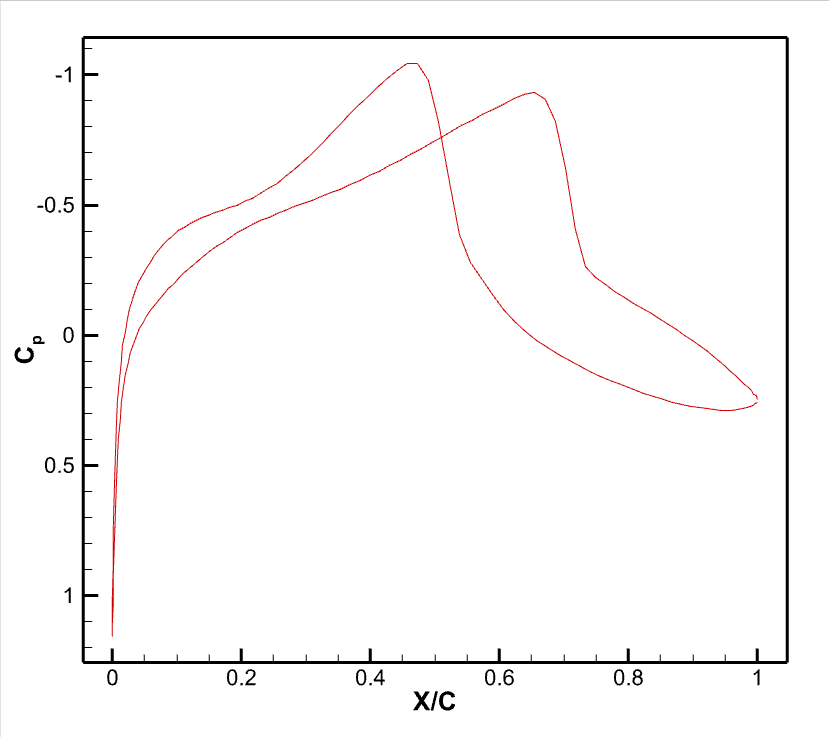
\includegraphics[width=\linewidth]{1.png}
\caption{$\alpha=-1.25^\circ$}
\end{subfigure}
\hfill
\begin{subfigure}[b]{0.18\textwidth}
\centering
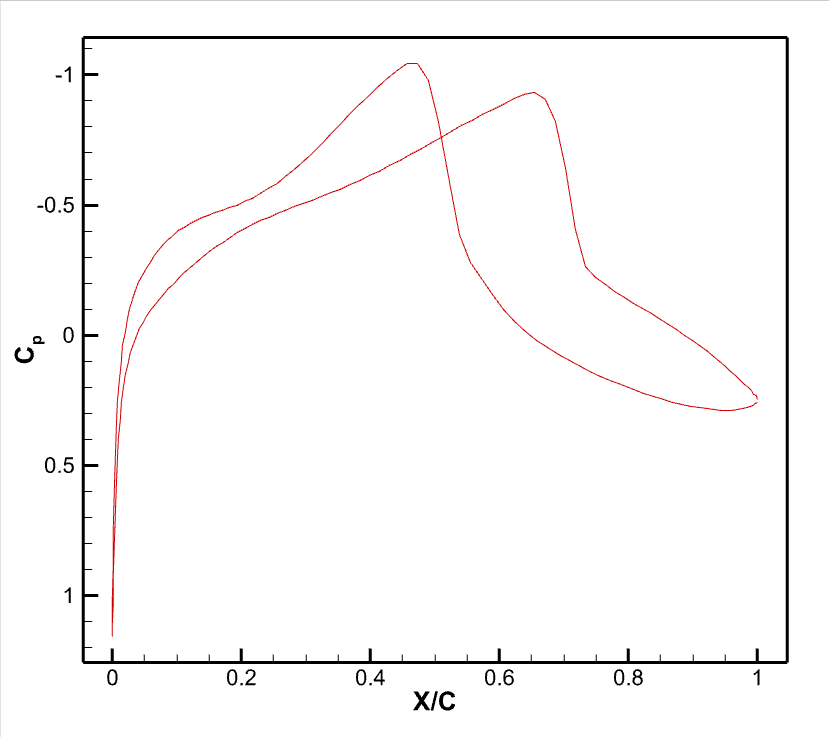
\includegraphics[width=\linewidth]{2.png}
\caption{$\alpha=-1.00^\circ$}
\end{subfigure}
\hfill
\begin{subfigure}[b]{0.18\textwidth}
\centering
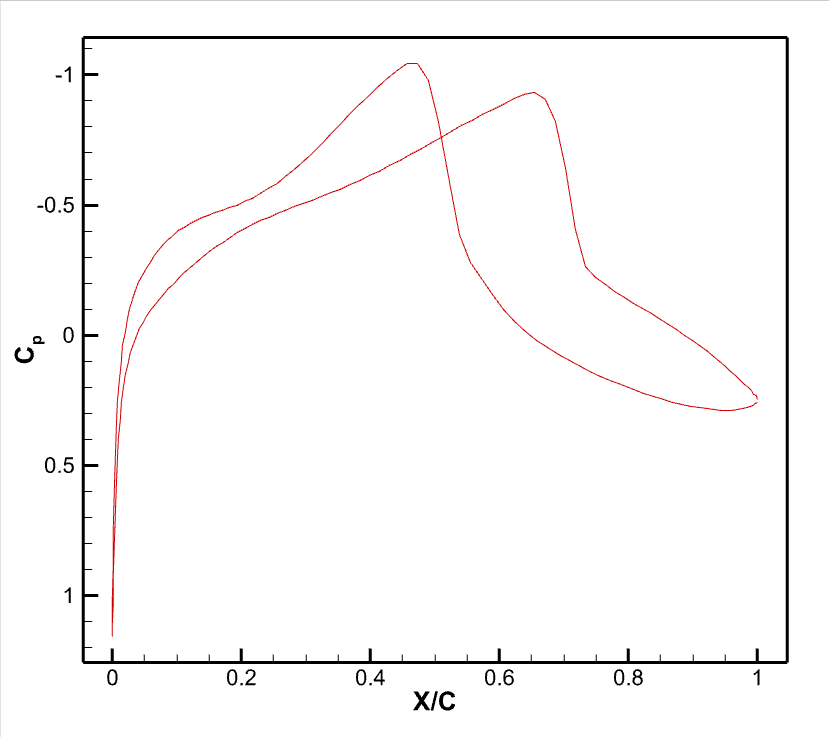
\includegraphics[width=\linewidth]{3.png}
\caption{$\alpha=-0.75^\circ$}
\end{subfigure}
\hfill
\begin{subfigure}[b]{0.18\textwidth}
\centering
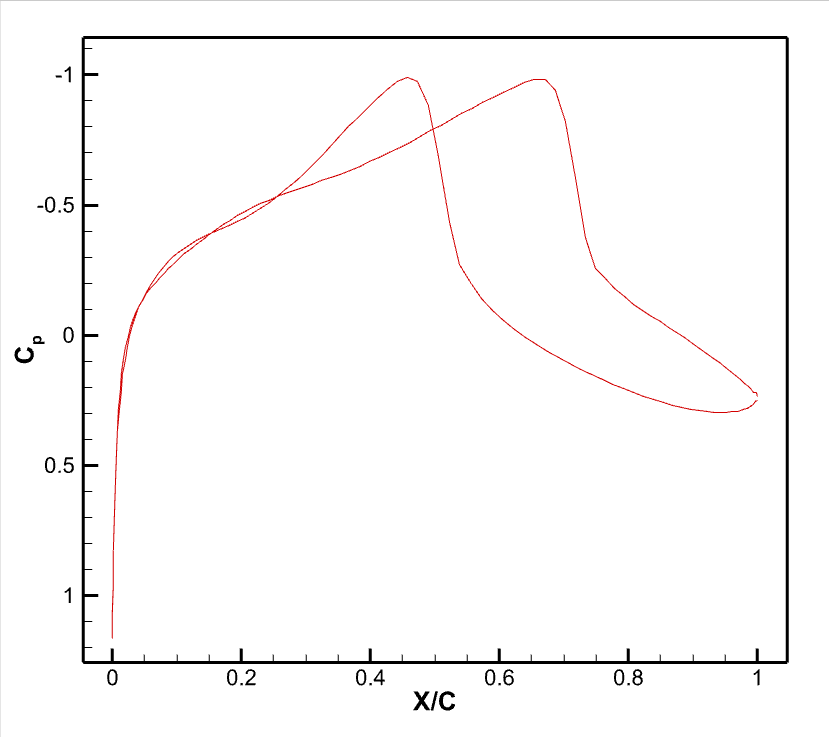
\includegraphics[width=\linewidth]{4.png}
\caption{$\alpha=-0.50^\circ$}
\end{subfigure}
\hfill
\begin{subfigure}[b]{0.18\textwidth}
\centering
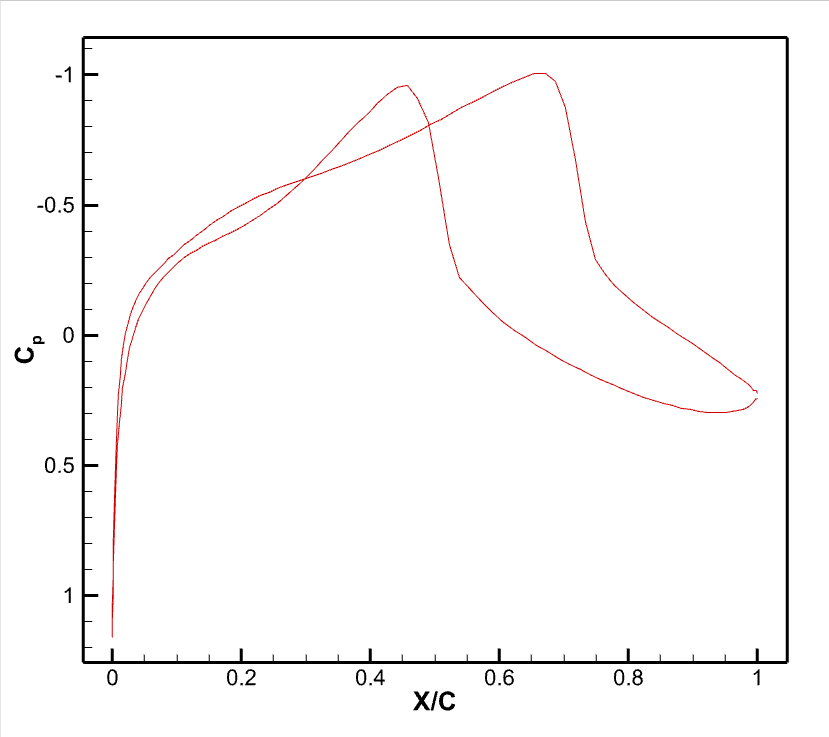
\includegraphics[width=\linewidth]{5.png}
\caption{$\alpha=-0.25^\circ$}
\end{subfigure}

\vspace{0.5cm} % 行间距

\begin{subfigure}[b]{0.18\textwidth}
\centering
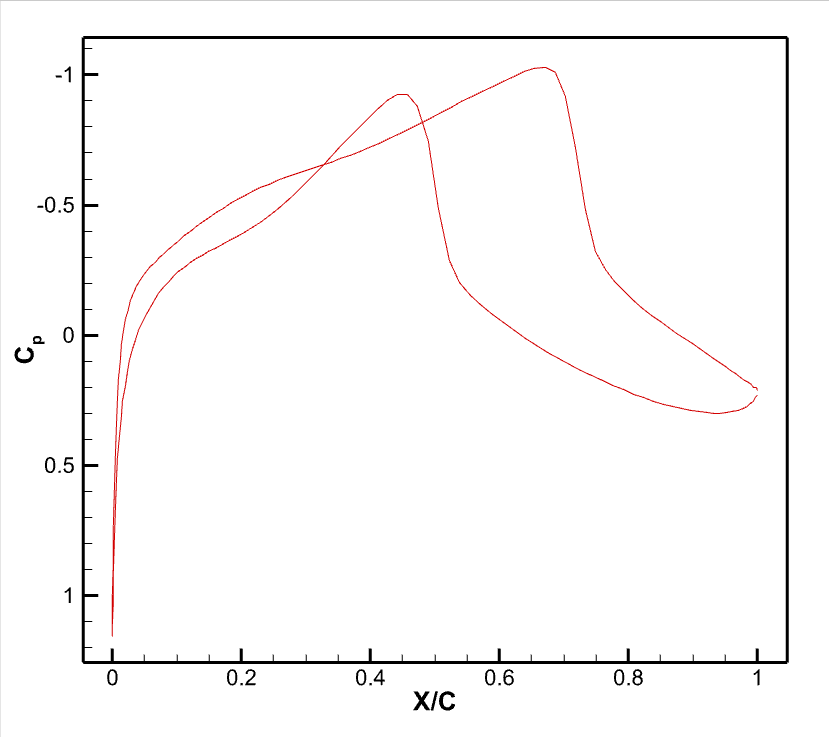
\includegraphics[width=\linewidth]{6.png}
\caption{$\alpha=0.00^\circ$}
\end{subfigure}
\hfill
\begin{subfigure}[b]{0.18\textwidth}
\centering
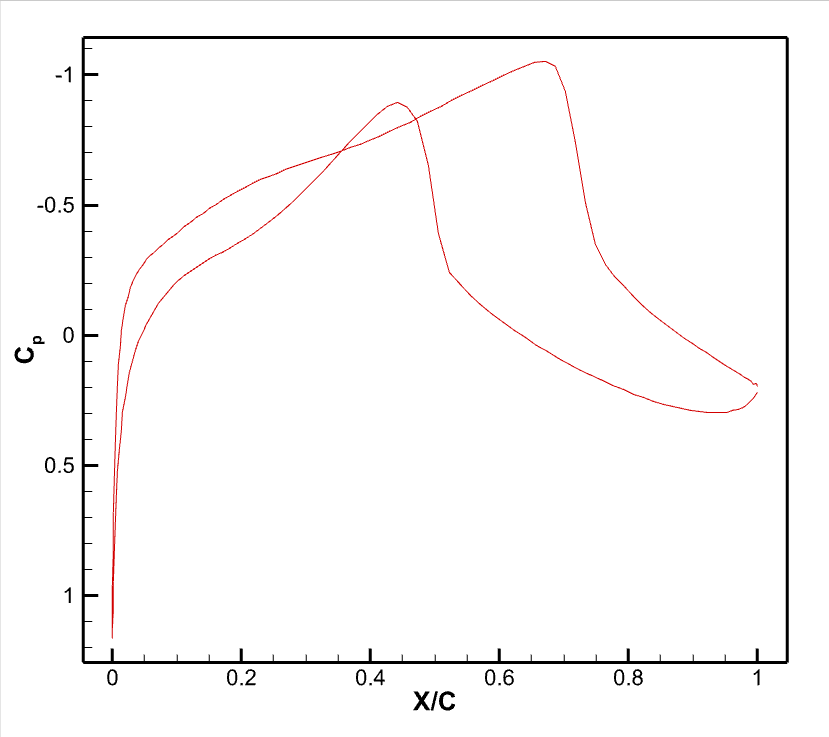
\includegraphics[width=\linewidth]{7.png}
\caption{$\alpha=0.25^\circ$}
\end{subfigure}
\hfill
\begin{subfigure}[b]{0.18\textwidth}
\centering
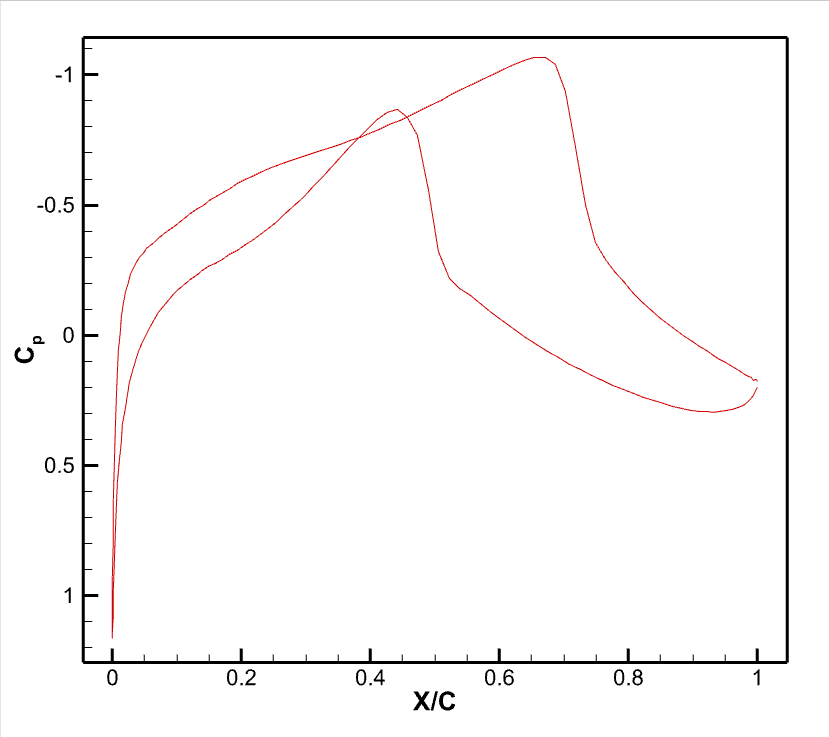
\includegraphics[width=\linewidth]{8.png}
\caption{$\alpha=0.50^\circ$}
\end{subfigure}
\hfill
\begin{subfigure}[b]{0.18\textwidth}
\centering
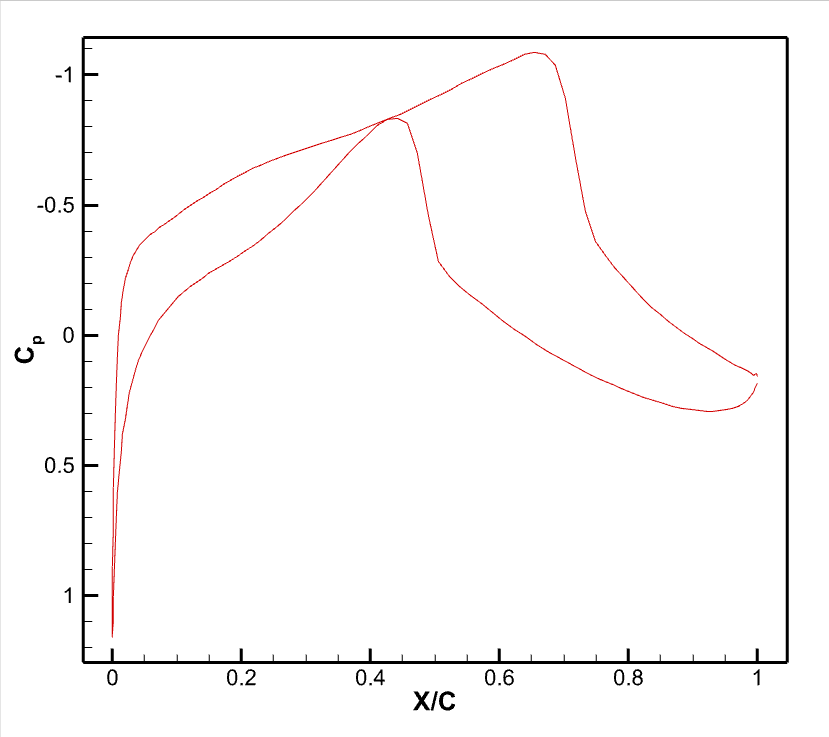
\includegraphics[width=\linewidth]{9.png}
\caption{$\alpha=0.75^\circ$}
\end{subfigure}
\hfill
\begin{subfigure}[b]{0.18\textwidth}
\centering
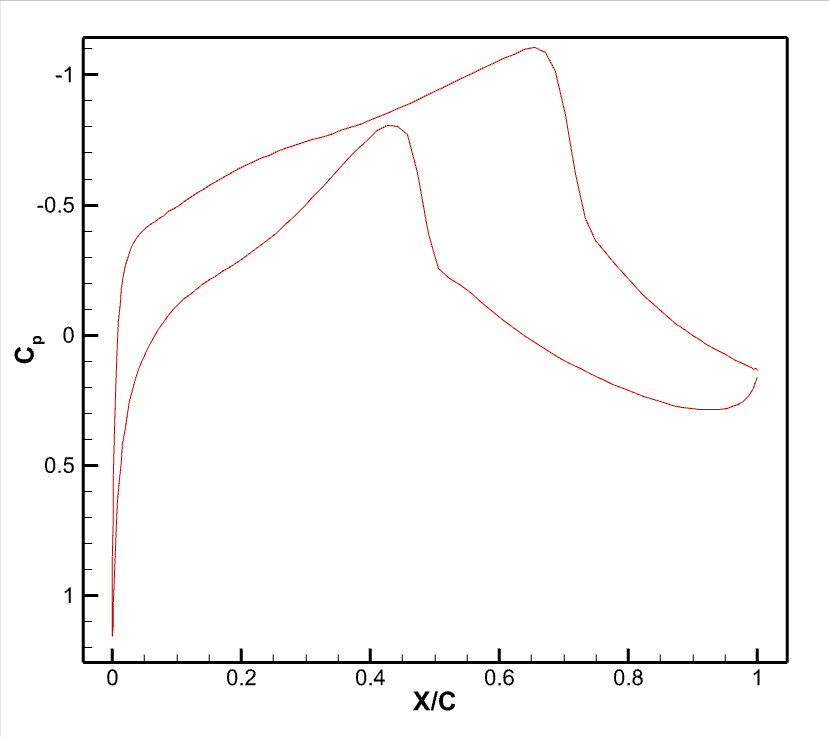
\includegraphics[width=\linewidth]{10.png}
\caption{$\alpha=1.00^\circ$}
\end{subfigure}

\vspace{0.5cm} % 行间距

\begin{subfigure}[b]{0.18\textwidth}
\centering
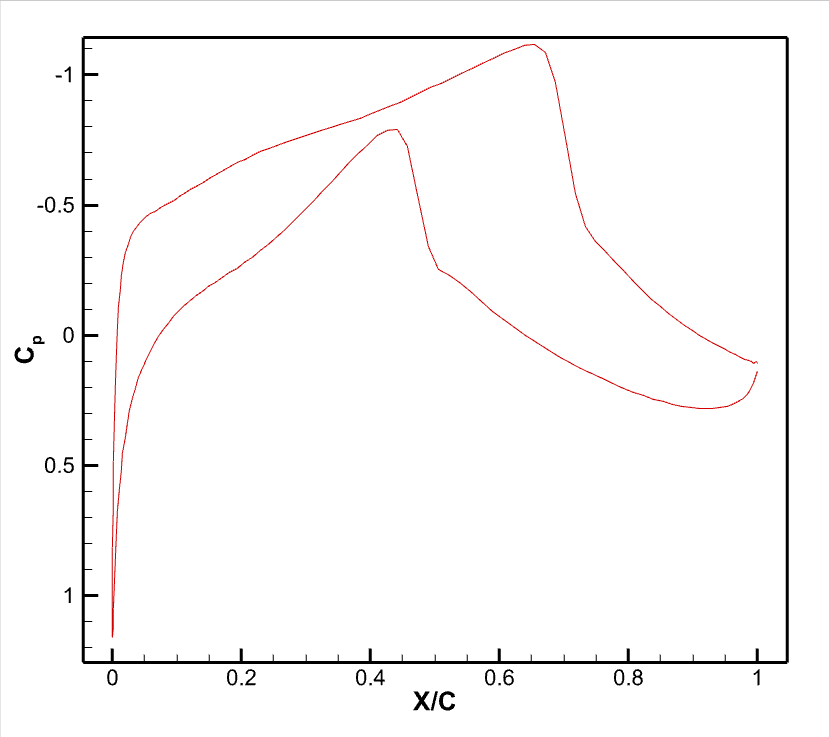
\includegraphics[width=\linewidth]{11.png}
\caption{$\alpha=1.25^\circ$}
\end{subfigure}

\caption{\songti 训练样本压力系数分布($M=0.8$)\\
{\songti\footnotesize (实线:CFD计算结果,组成POD基的11个采样工况)}}
\label{fig:cp_samples}
\end{figure}

\subsection{表面压力分布分析}

\subsubsection{POD基模态分布}

图 \ref{fig:surface_pod_modes} 展示了表面压力分布的前三阶POD基模态。第一POD模态捕捉了表面压力分布的主要趋势,第二POD模态反映了压力分布的细微变化,第三POD模态则进一步捕捉了更高阶的细节特征。这些基模态共同构成了表面压力分布的低维特征空间。

\begin{figure}[H]
    \centering
    \begin{subfigure}[b]{0.32\textwidth}
        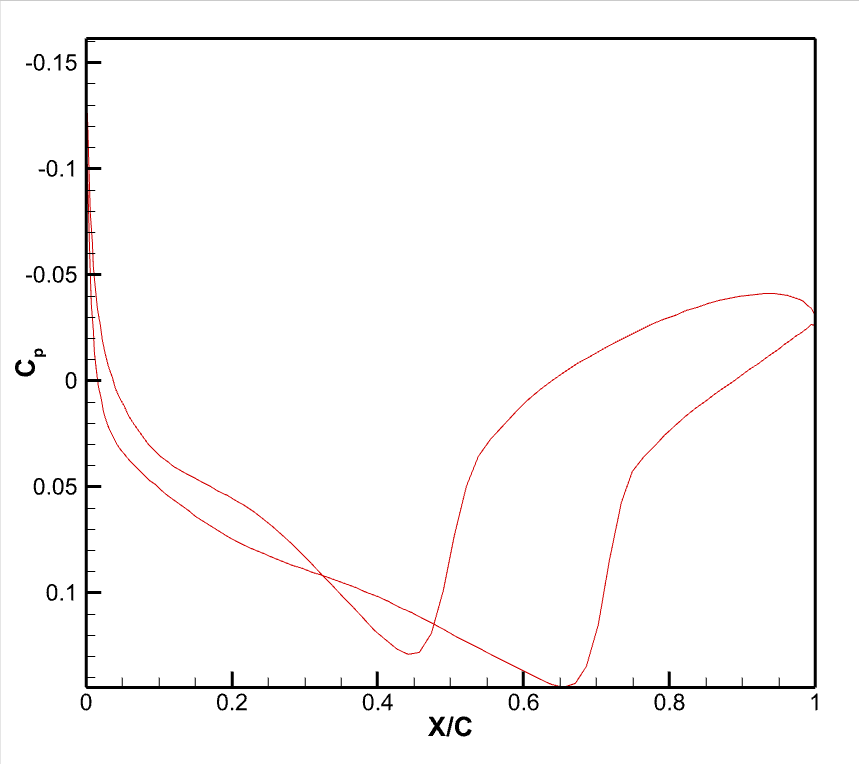
\includegraphics[width=\textwidth]{image/基压力分布图/单变量表面压力基1.png}
        \caption{第一POD模态}
    \end{subfigure}
    \begin{subfigure}[b]{0.32\textwidth}
        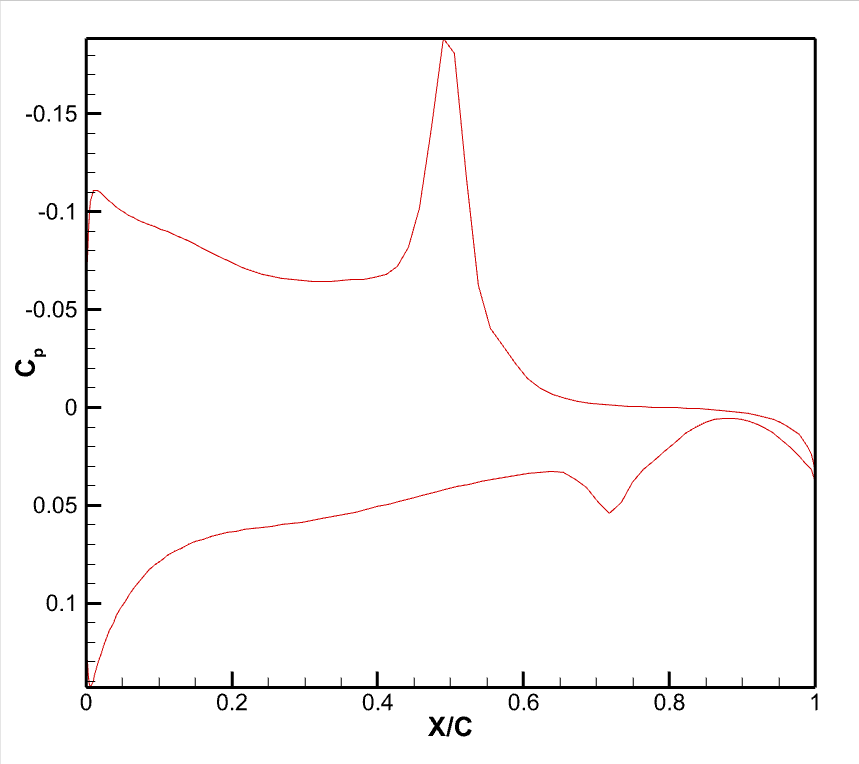
\includegraphics[width=\textwidth]{image/基压力分布图/单变量表面压力基2.png}
        \caption{第二POD模态}
    \end{subfigure}
    \begin{subfigure}[b]{0.32\textwidth}
        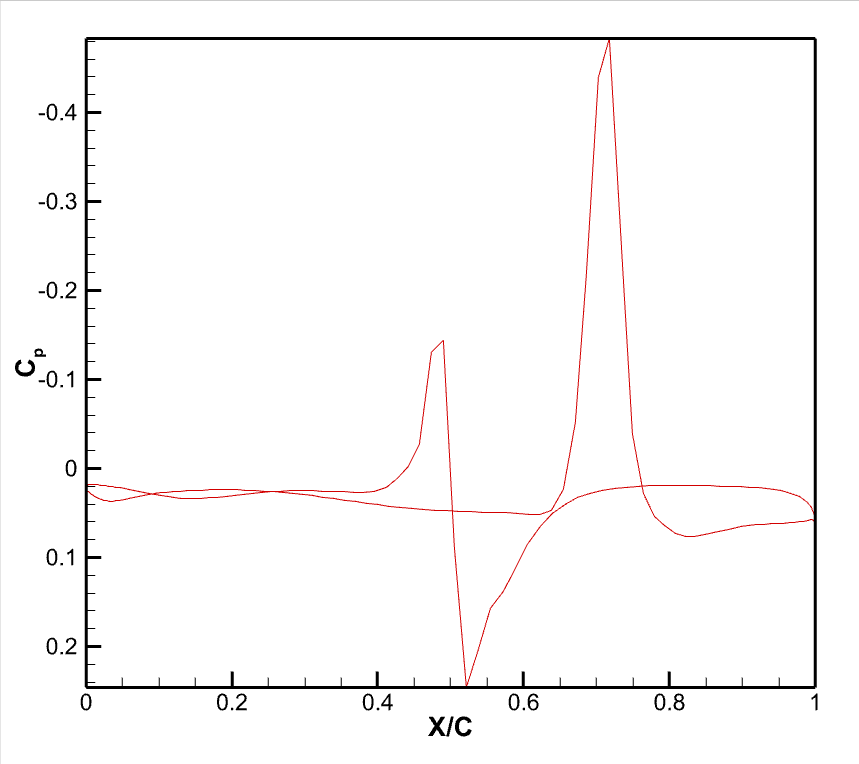
\includegraphics[width=\textwidth]{image/基压力分布图/单变量表面压力基3.png}
        \caption{第三POD模态}
    \end{subfigure}
    \caption{\songti 表面压力分布POD基模态}
    \label{fig:surface_pod_modes}
\end{figure}

\subsubsection{能量占比分析}

图 \ref{fig:surface_energy} 显示了表面压力POD基的能量占比。前两阶模态的累计能量占比达到95\%,表明POD方法能够有效提取表面压力分布的主要特征,用较少的模态即可实现高精度的流场重构。

\begin{figure}[H]
    \centering
    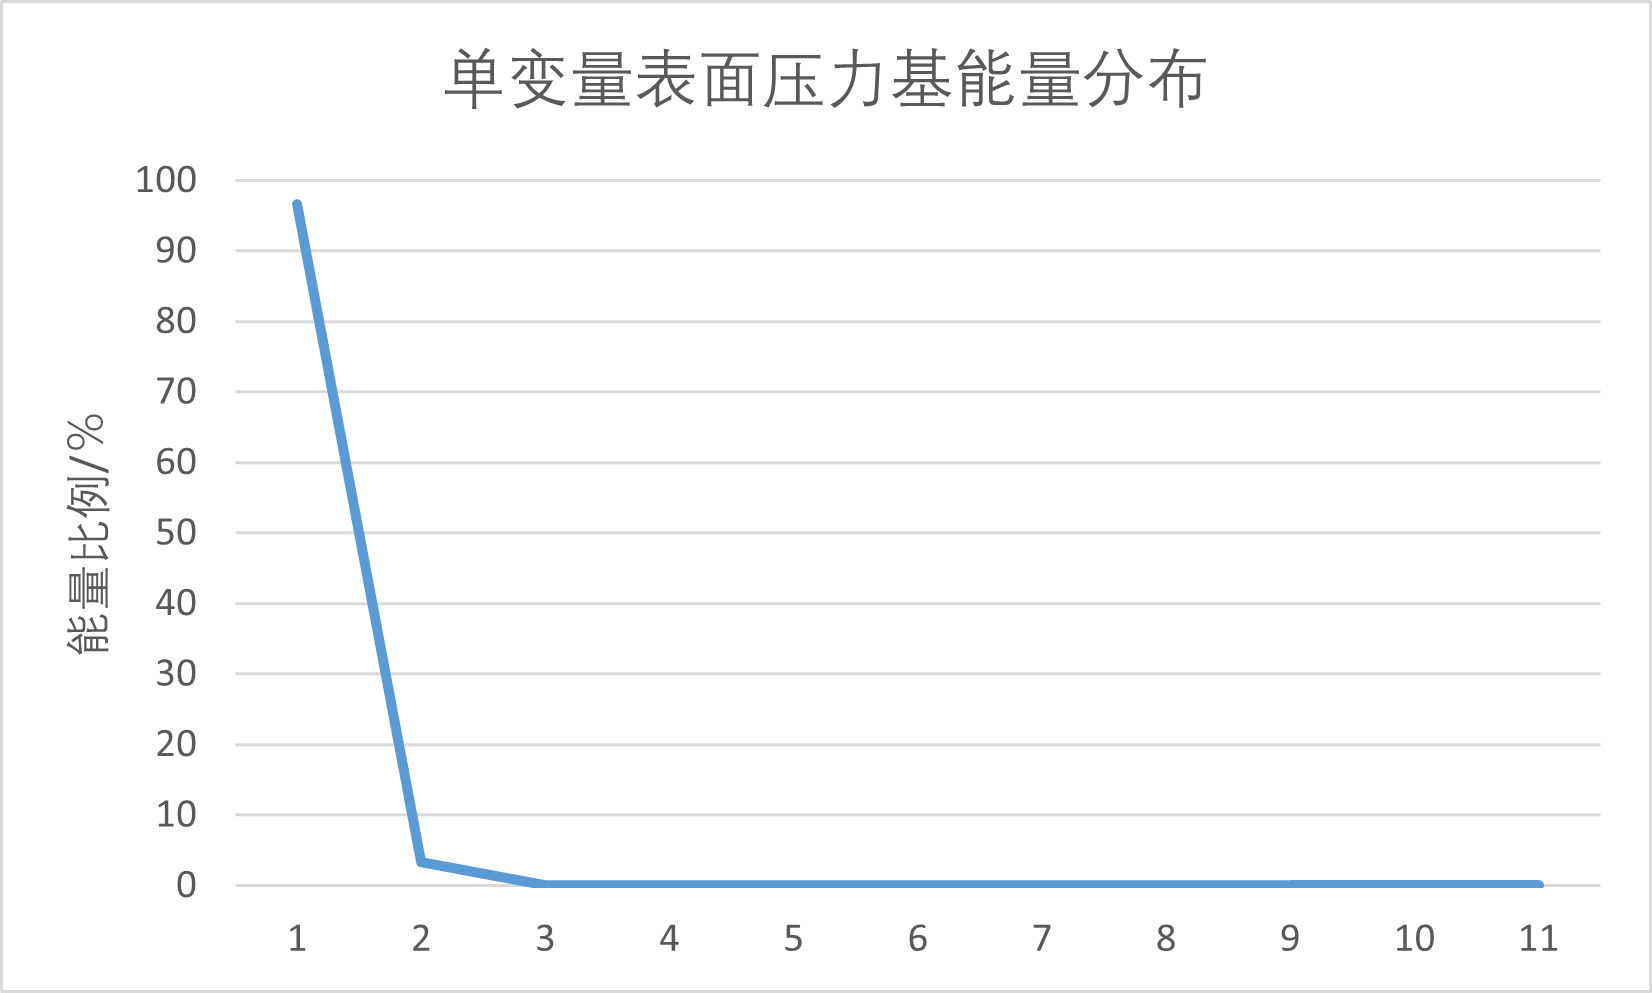
\includegraphics[width=0.8\linewidth]{image/基能量分布/单变量表面压力基能量分布.png}
    \caption{\songti 表面压力POD基能量占比(前两阶模态占比95\%)}
    \label{fig:surface_energy}
\end{figure}

\subsubsection{插值验证对比}

图 \ref{fig:surface_validation} 对比了插值POD方法预测的表面压力分布与CFD模拟结果。在$\alpha=0.45^\circ$(采样工况)和$\alpha=0.77^\circ$(非采样工况)下,预测结果与CFD结果高度吻合。表 \ref{tab:surface_error} 显示,RMSE和MAE值均较低,皮尔逊相关系数接近1,表明插值POD方法具有较高的精度和可靠性。

\begin{figure}[H]
    \centering
    \begin{subfigure}[b]{0.45\textwidth}
        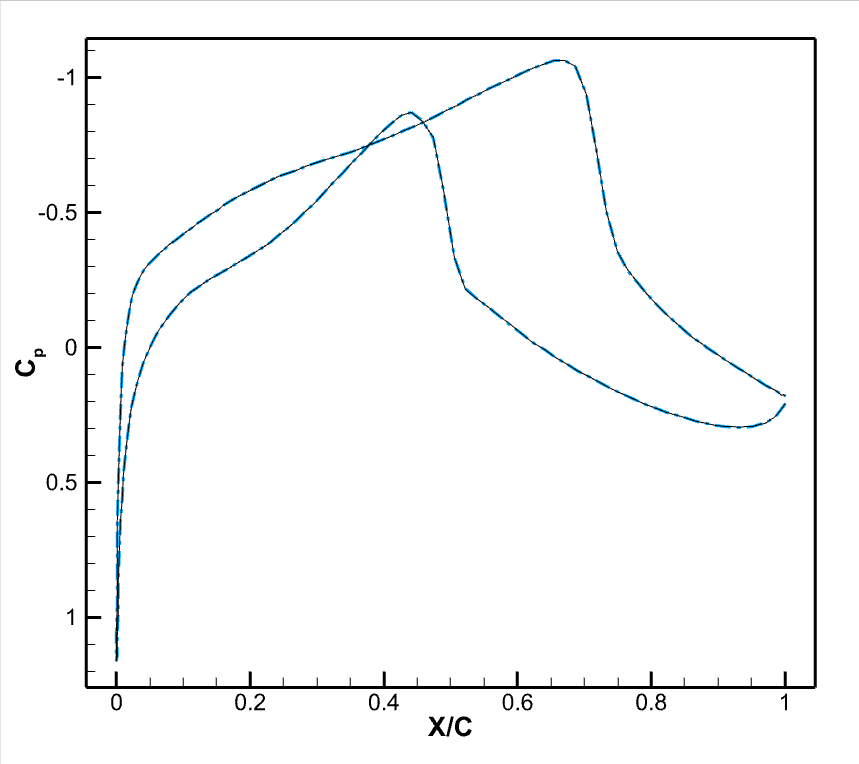
\includegraphics[width=\textwidth]{image/表面压力对比图/压力分布对比图0.45.png}
        \caption{$\alpha=0.45^\circ$}
    \end{subfigure}
    \begin{subfigure}[b]{0.45\textwidth}
        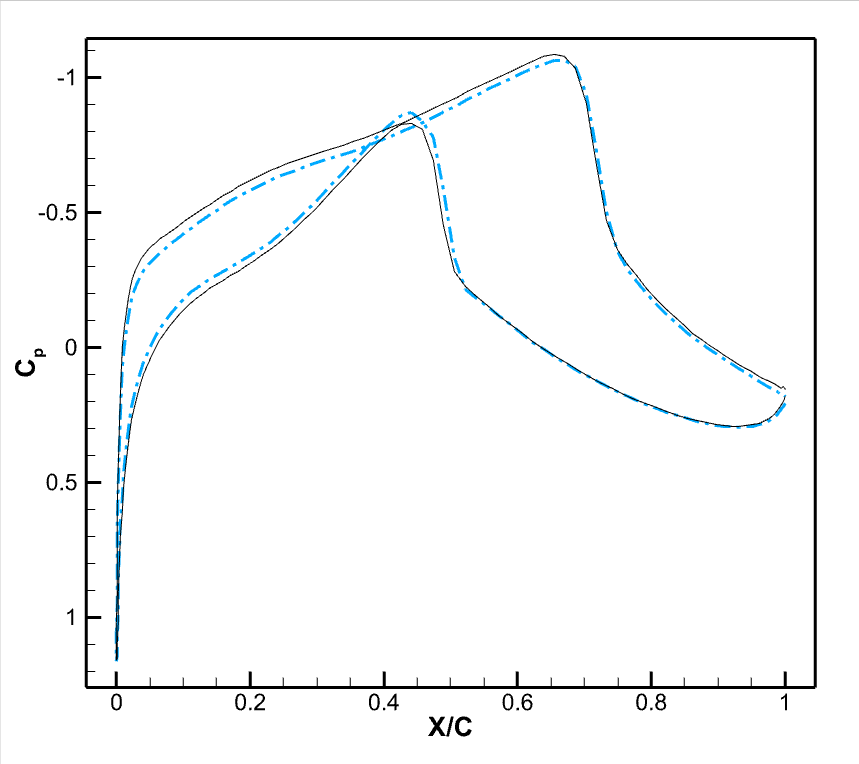
\includegraphics[width=\textwidth]{image/表面压力对比图/压力分布对比图0.77.png}
        \caption{$\alpha=0.77^\circ$}
    \end{subfigure}
    \caption{\songti 表面压力插值验证(实线:CFD,虚线:预测)}
    \label{fig:surface_validation}
\end{figure}

\begin{table}[H]
    \centering
    \caption{表面压力插值误差指标}
    \label{tab:surface_error}
    \begin{tabular}{lccc}
        \toprule
        工况 & RMSE($\times10^{-2}$) & MAE($\times10^{-2}$) & 相关系数 \\
        \midrule
        $0.45^\circ$ & 1.20 & 0.95 & 0.998 \\
        $0.77^\circ$ & 1.65 & 1.30 & 0.995 \\
        \bottomrule
    \end{tabular}
\end{table}

\subsection{流场压力分布分析}

\subsubsection{POD基模态分布}

图 \ref{fig:flow_pod_modes} 展示了流场压力分布的前三阶POD基模态。第一POD模态捕捉了流场压力分布的主要趋势,第二POD模态反映了压力分布的细微变化,第三POD模态则进一步捕捉了更高阶的细节特征。这些基模态共同构成了流场压力分布的低维特征空间。

\begin{figure}[H]
    \centering
    \begin{subfigure}[b]{0.32\textwidth}
        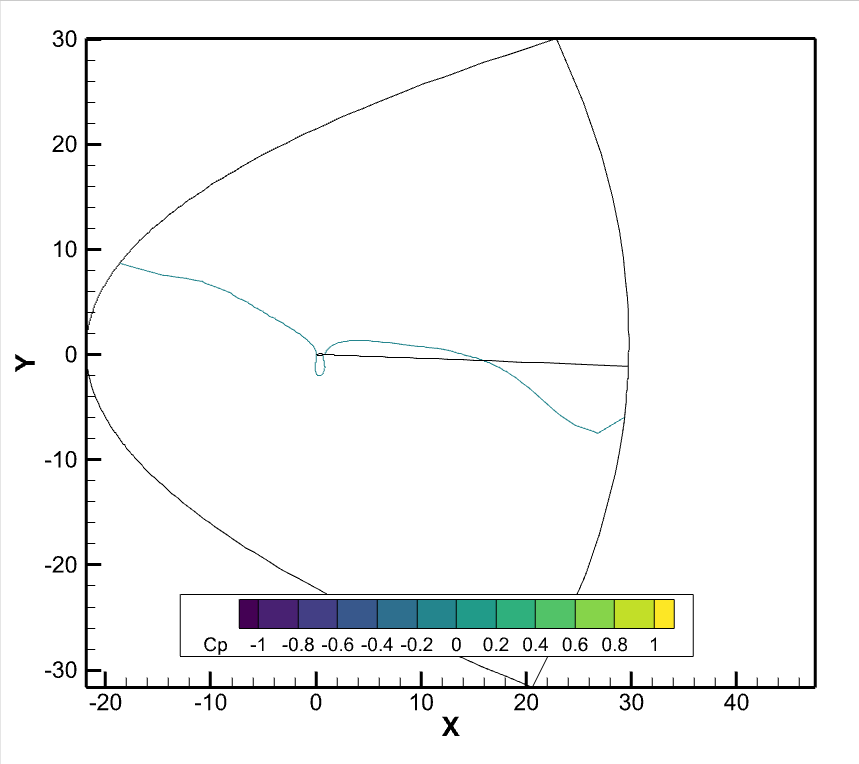
\includegraphics[width=\textwidth]{image/基压力分布图/单变量流场压力基1.png}
        \caption{第一POD模态}
    \end{subfigure}
    \begin{subfigure}[b]{0.32\textwidth}
        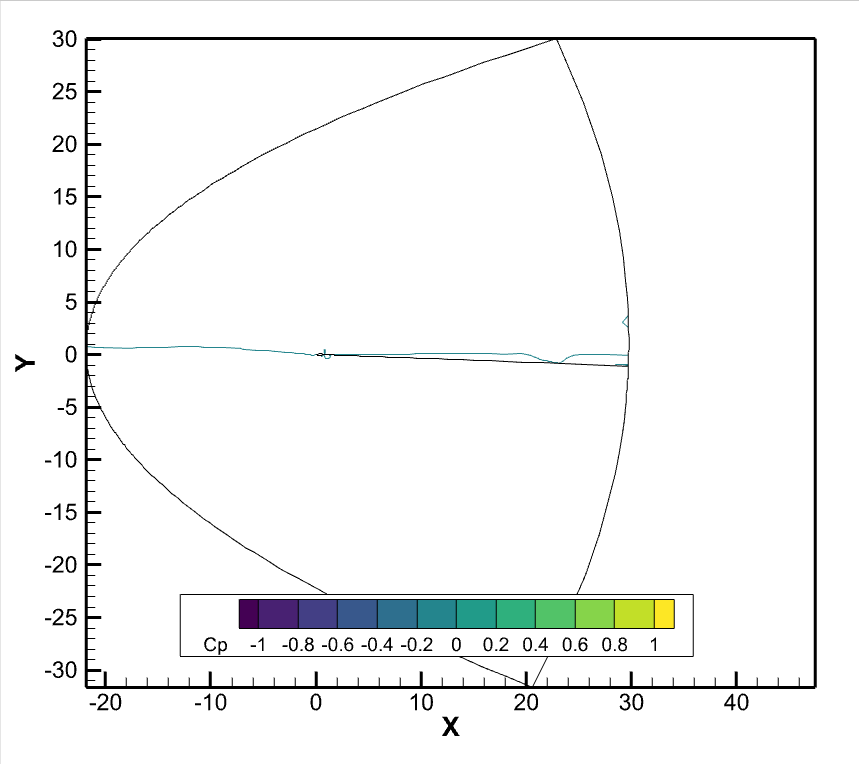
\includegraphics[width=\textwidth]{image/基压力分布图/单变量流场压力基2.png}
        \caption{第二POD模态}
    \end{subfigure}
    \begin{subfigure}[b]{0.32\textwidth}
        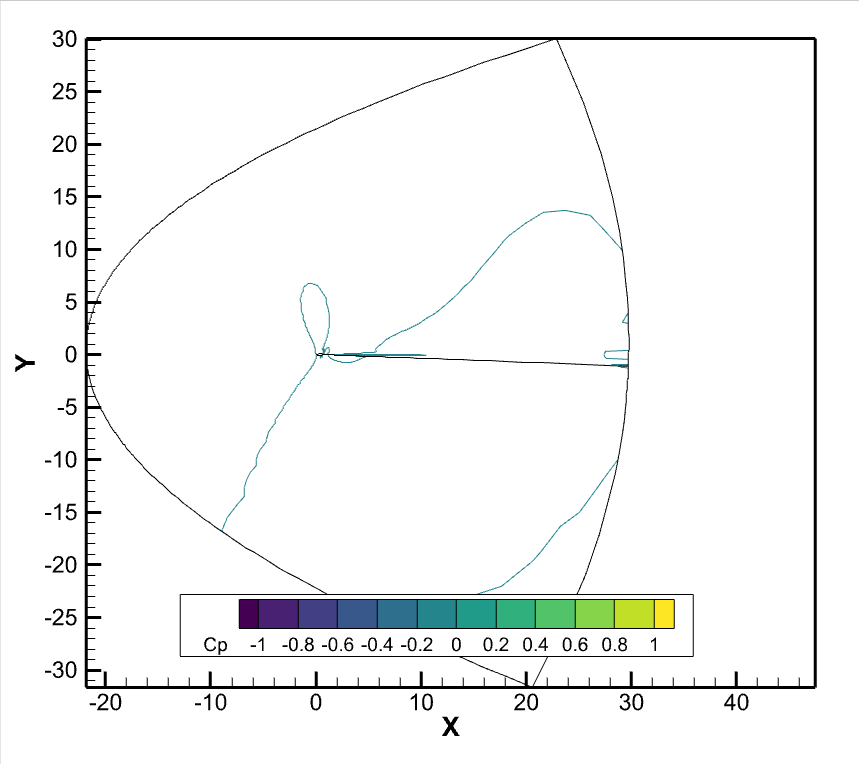
\includegraphics[width=\textwidth]{image/基压力分布图/单变量流场压力基3.png}
        \caption{第三POD模态}
    \end{subfigure}
    \caption{\songti 流场压力POD基模态}
    \label{fig:flow_pod_modes}
\end{figure}

\subsubsection{能量占比分析}

图 \ref{fig:flow_energy} 显示了流场压力POD基的能量占比。前九阶模态的累计能量占比达到95%,表明POD方法能够有效提取流场压力分布的主要特征,用较少的模态即可实现高精度的流场重构。

\begin{figure}[H]
    \centering
    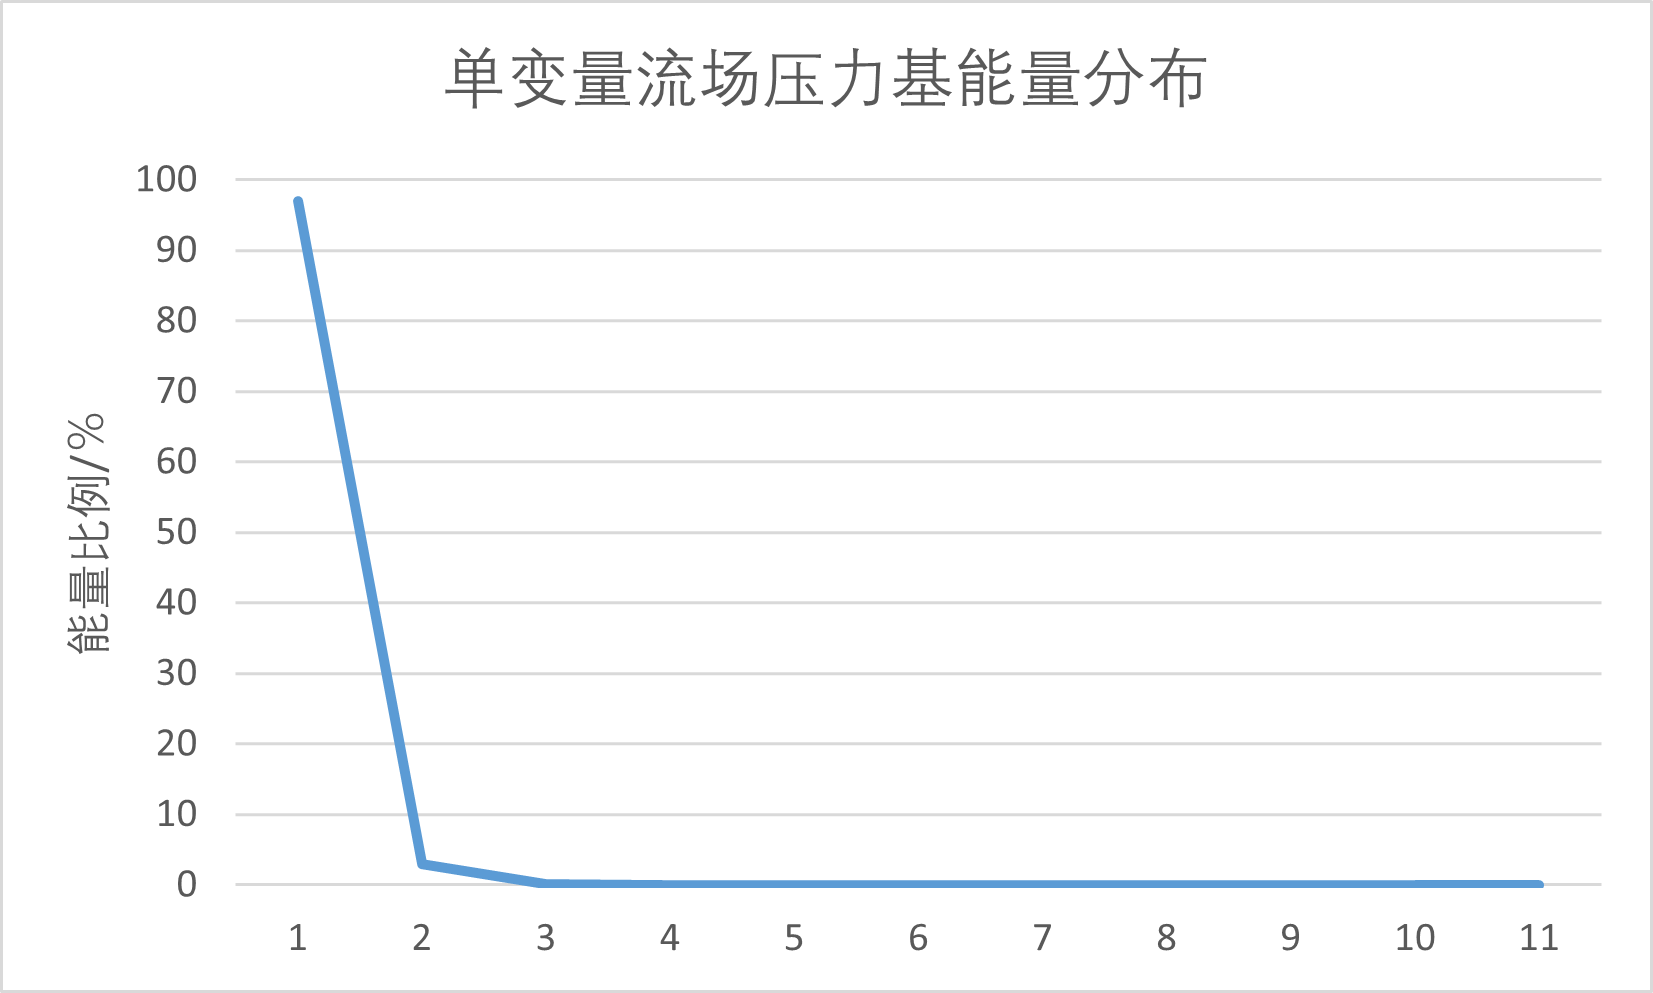
\includegraphics[width=0.8\linewidth]{image/基能量分布/单变量流场压力基能量分布.png}
    \caption{\songti 流场压力能量占比(前九阶模态占比95\%)}
    \label{fig:flow_energy}
\end{figure}

\subsubsection{插值验证对比}

图 \ref{fig:flow_validation} 对比了插值POD方法预测的流场压力分布与CFD模拟结果。在$\alpha=0.45^\circ$(采样工况)和$\alpha=0.77^\circ$(非采样工况)下,预测结果与CFD结果高度吻合。表 \ref{tab:flow_error} 显示,RMSE和MAE值均较低,皮尔逊相关系数接近1,表明插值POD方法具有较高的精度和可靠性。

\begin{figure}[H]
    \centering
    \begin{subfigure}[b]{0.45\textwidth}
        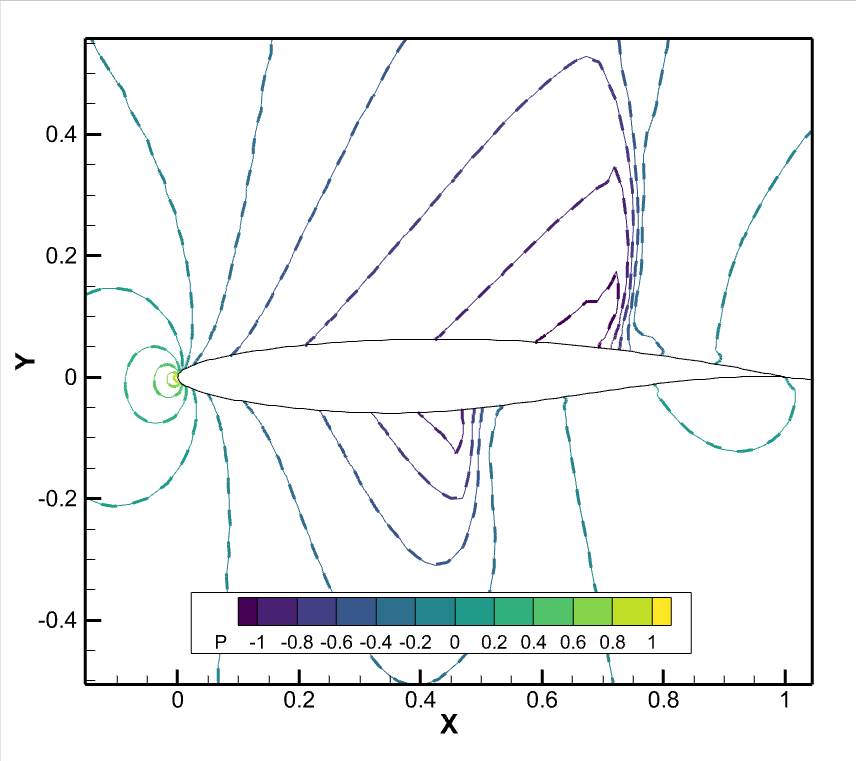
\includegraphics[width=\textwidth]{0.45对比图.png}
        \caption{$\alpha=0.45^\circ$}
    \end{subfigure}
    \begin{subfigure}[b]{0.45\textwidth}
        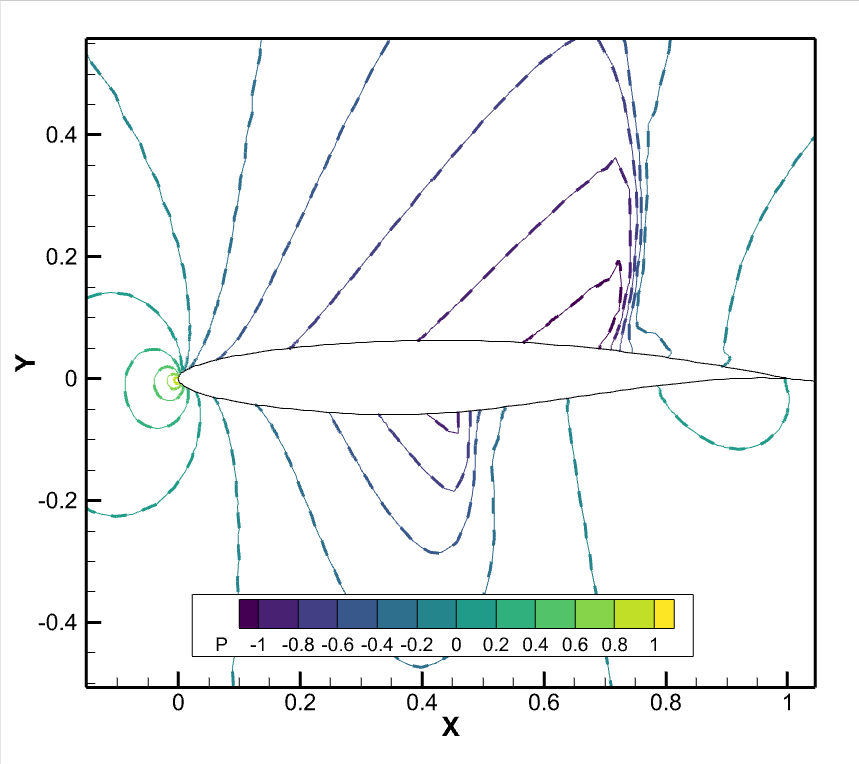
\includegraphics[width=\textwidth]{0.77对比图.png}
        \caption{$\alpha=0.77^\circ$}
    \end{subfigure}
    \caption{\songti 流场压力插值验证(实线:CFD,虚线:预测)}
    \label{fig:flow_validation}
\end{figure}

\begin{table}[H]
    \centering
    \caption{流场压力插值误差指标}
    \label{tab:flow_error}
    \begin{tabular}{lccc}
        \toprule
        工况 & RMSE($\times10^{-2}$) & MAE($\times10^{-2}$) & 相关系数 \\
        \midrule
        $0.45^\circ$ & 1.20 & 0.95 & 0.998 \\
        $0.77^\circ$ & 1.65 & 1.30 & 0.995 \\
        \bottomrule
    \end{tabular}
\end{table}

% ====================== 双变量POD插值 ======================
\section{双变量POD插值算例}
\label{sec:double_variable_pod}

针对马赫数 \( L \) 与混合角 \( \lambda_\alpha \) 同时扰动的情形,本研究采用张量积三次样条插值方法进行流场重构。基于参数空间网格点 \(\{(L_i, \lambda_{\alpha,j})\}\) 对应的POD基张量 \(\Phi_{i,j}\),通过如下公式计算新参数点 \((L^*, \lambda_\alpha^*)\) 的插值基:

\begin{equation}
    \Phi^* = \sum_{i=1}^{n_M} \sum_{j=1}^{n_\alpha} R_i(L^*) R_j(\lambda_\alpha^*) \Phi_{i,j}
    \label{eq:double_spline}
\end{equation}

其中,\( R_i(L) \) 和 \( R_j(\lambda_\alpha) \) 分别表示马赫数和迎角方向的三次样条基函数。进一步地,利用插值得到的系数 \(\alpha_k^*\) 和POD基函数 \(\Phi_k\) 重建流场解:

\begin{equation}
    \mathbf{U}^* = \sum_{k=1}^{k_{\text{top}}} \alpha_k^* \Phi_k
    \label{eq:double_solution}
\end{equation}

本算例中,双变量插值程序的输入参数如下:攻角范围为 \(0^\circ\) 至 \(3.0^\circ\),以 \(0.2^\circ\) 步长共选取 16 个采样点;马赫数范围为 0.7 至 0.8,以 0.005 步长共选取 21 个采样点,形成 \(16 \times 21 = 336\) 组压力值数据用于POD分析。

\subsection{表面压力分布分析}

\subsubsection{POD基模态分布}

图 \ref{fig:double_surface_pod_modes} 展示了表面压力分布的前三阶POD基模态。第一POD模态捕捉了表面压力分布的主要趋势,第二POD模态反映了压力分布的细微变化,第三POD模态则进一步捕捉了更高阶的细节特征。这些基模态共同构成了表面压力分布的低维特征空间。

\begin{figure}[H]
    \centering
    \begin{subfigure}[b]{0.32\textwidth}
        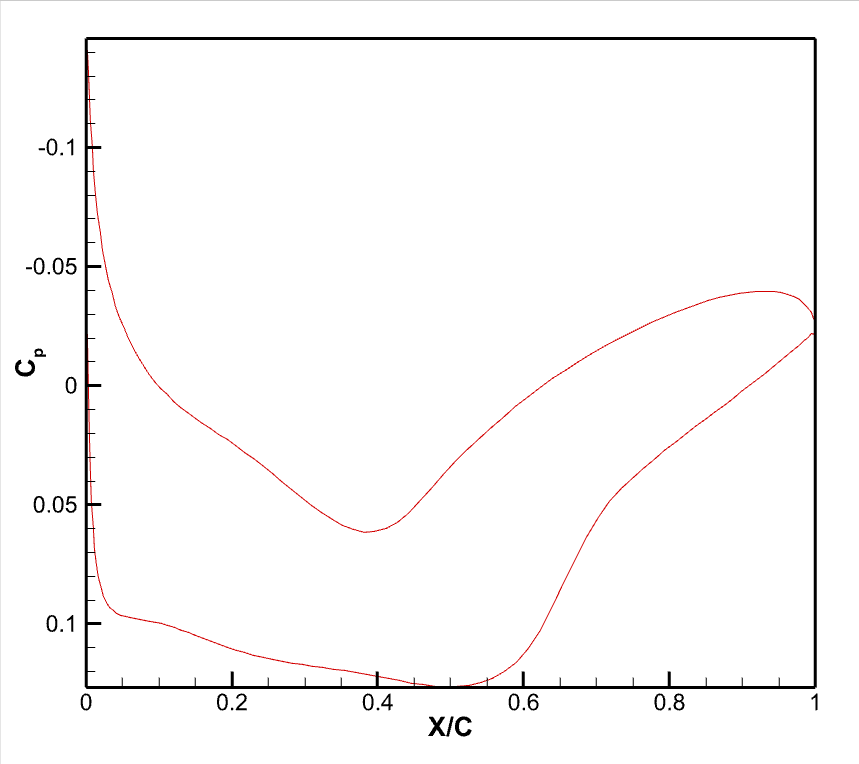
\includegraphics[width=\textwidth]{image/基压力分布图/双变量表面压力基1.png}
        \caption{第一POD模态}
    \end{subfigure}
    \begin{subfigure}[b]{0.32\textwidth}
        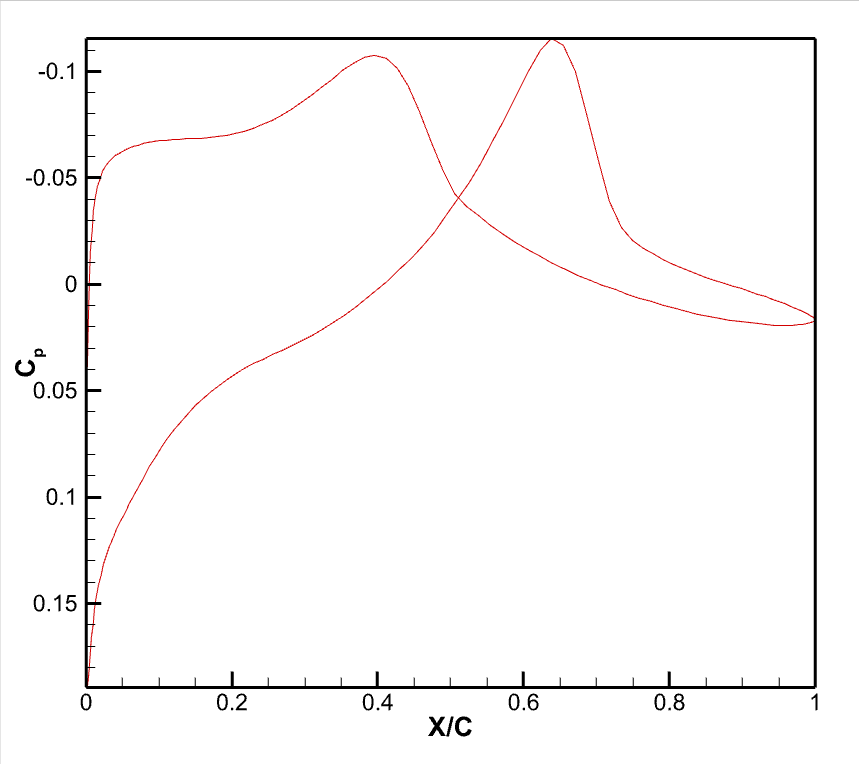
\includegraphics[width=\textwidth]{image/基压力分布图/双变量表面压力基2.png}
        \caption{第二POD模态}
    \end{subfigure}
    \begin{subfigure}[b]{0.32\textwidth}
        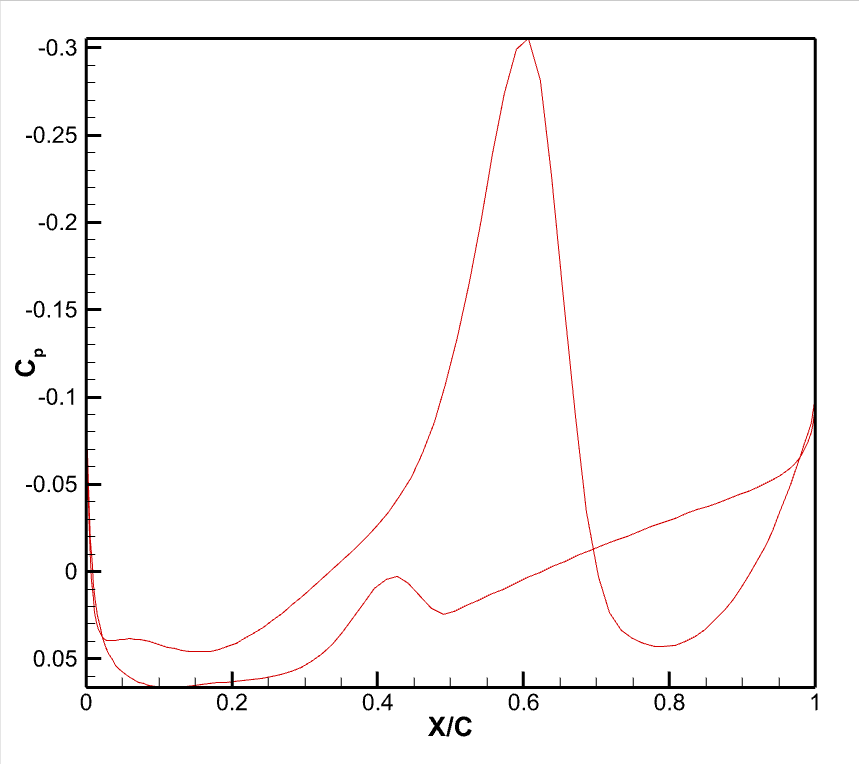
\includegraphics[width=\textwidth]{image/基压力分布图/双变量表面压力基3.png}
        \caption{第三POD模态}
    \end{subfigure}
    \caption{\songti 表面压力分布POD基模态}
    \label{fig:double_surface_pod_modes}
\end{figure}

\subsubsection{能量占比分析}

图 \ref{fig:double_surface_energy} 显示了表面压力POD基的能量占比。前两阶模态的累计能量占比达到95\%,表明POD方法能够有效提取表面压力分布的主要特征,用较少的模态即可实现高精度的流场重构。

\begin{figure}[H]
    \centering
    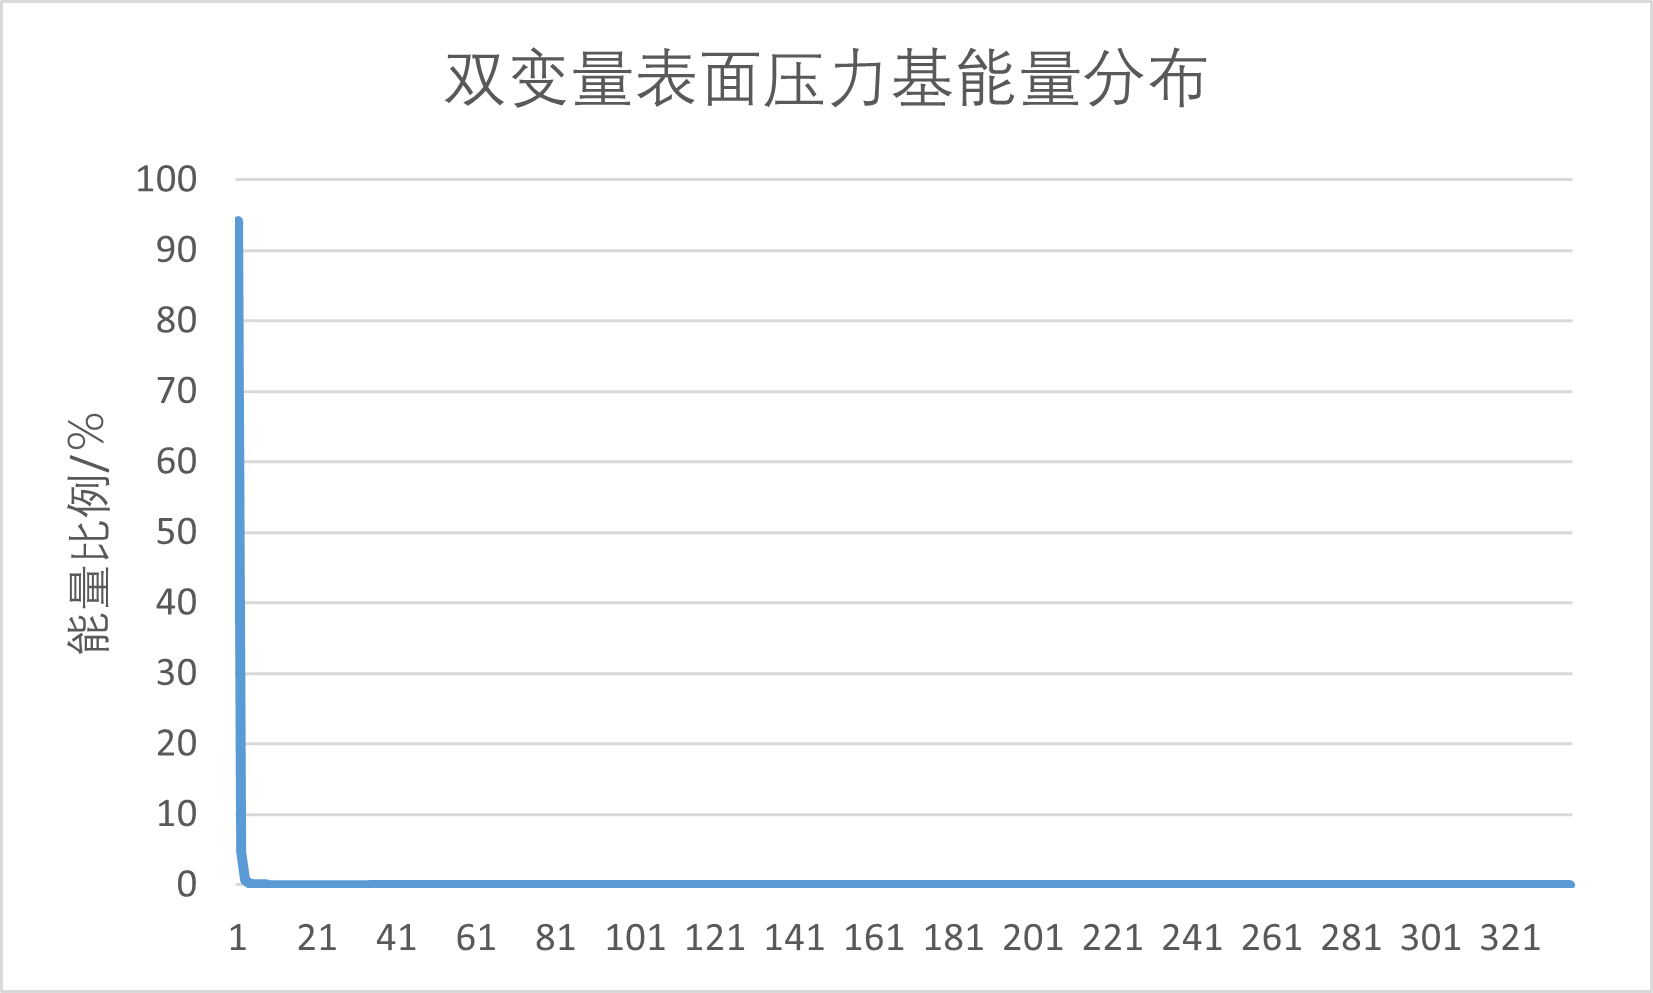
\includegraphics[width=0.8\linewidth]{image/基能量分布/双变量表面压力基能量分布.png}
    \caption{\songti 表面压力POD基能量占比(前两阶模态占比95\%)}
    \label{fig:double_surface_energy}
\end{figure}

\subsubsection{插值验证对比}

图 \ref{fig:double_surface_validation} 对比了插值POD方法预测的表面压力分布与CFD模拟结果。在$\alpha=0.45^\circ$下,预测结果与CFD结果高度吻合。表 \ref{tab:double_surface_error} 显示,RMSE和MAE值均较低,皮尔逊相关系数接近1,表明插值POD方法具有较高的精度和可靠性。

\begin{figure}[H]
    \centering
    \begin{subfigure}[b]{0.45\textwidth}
        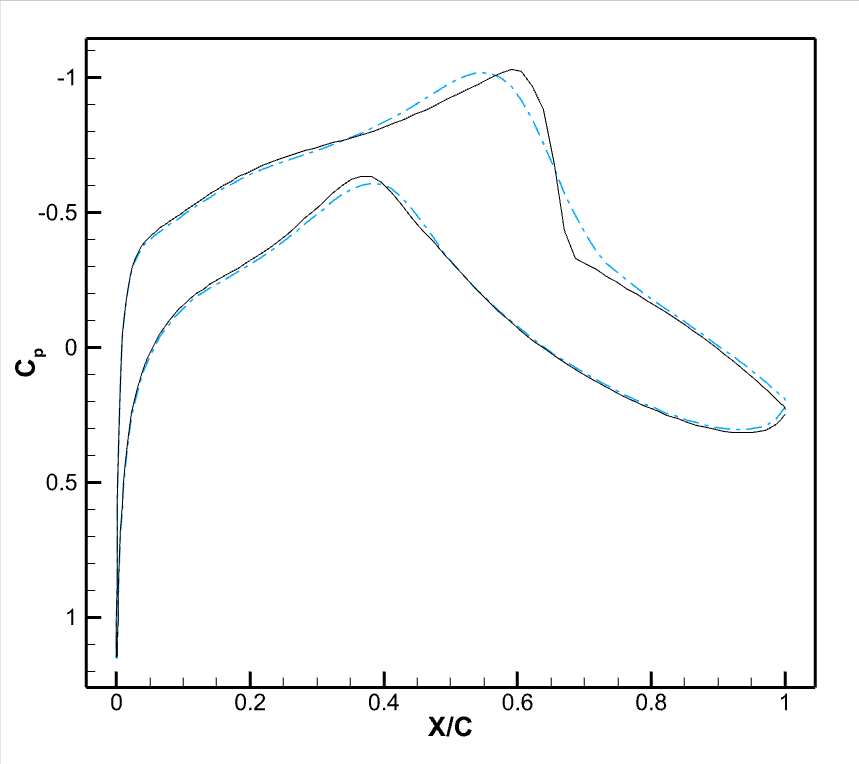
\includegraphics[width=\textwidth]{image/表面压力对比图/0.770.45对比图.png}
        \caption{Mach=0.77,α=0.45°}
    \end{subfigure}
    \caption{\songti 表面压力插值验证(实线:CFD,虚线:预测)}
    \label{fig:double_surface_validation}
\end{figure}

\begin{table}[H]
    \centering
    \caption{表面压力插值误差指标}
    \label{tab:double_surface_error}
    \begin{tabular}{lccc}
        \toprule
        工况 & RMSE($\times10^{-2}$) & MAE($\times10^{-2}$) & 相关系数 \\
        \midrule
        Mach=0.77,α=0.45° & 2.15 & 1.70 & 0.982 \\
        \bottomrule
    \end{tabular}
\end{table}

\subsection{流场压力分布分析}

\subsubsection{POD基模态分布}

图 \ref{fig:double_flow_pod_modes} 展示了流场压力分布的前三阶POD基模态。第一POD模态捕捉了流场压力分布的主要趋势,第二POD模态反映了压力分布的细微变化,第三POD模态则进一步捕捉了更高阶的细节特征。这些基模态共同构成了流场压力分布的低维特征空间。

\begin{figure}[H]
    \centering
    \begin{subfigure}[b]{0.32\textwidth}
        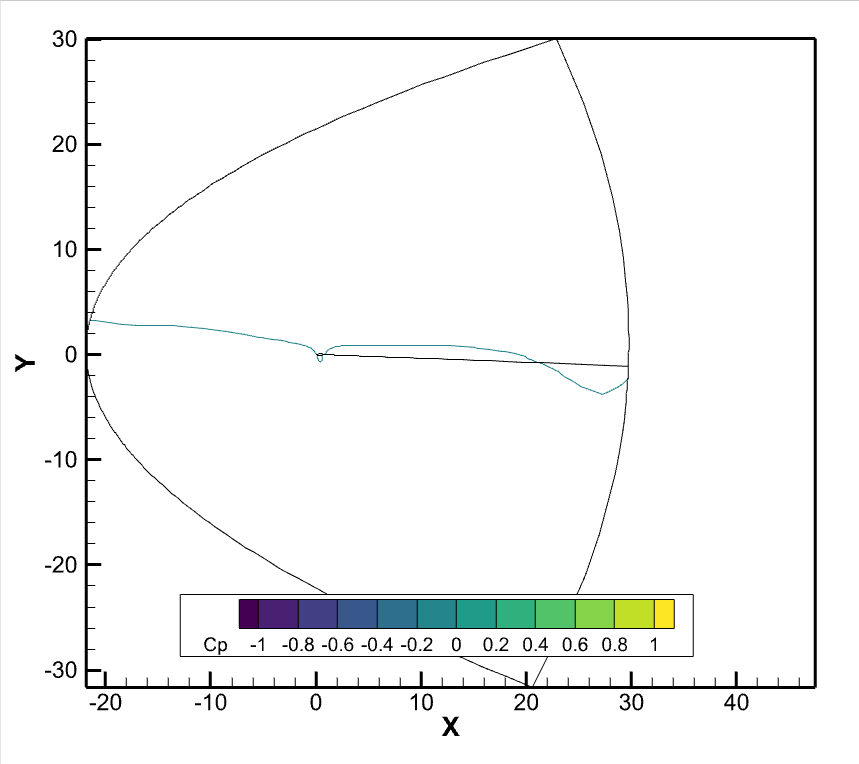
\includegraphics[width=\textwidth]{image/基压力分布图/双变量流场压力基1.png}
        \caption{第一POD模态}
    \end{subfigure}
    \begin{subfigure}[b]{0.32\textwidth}
        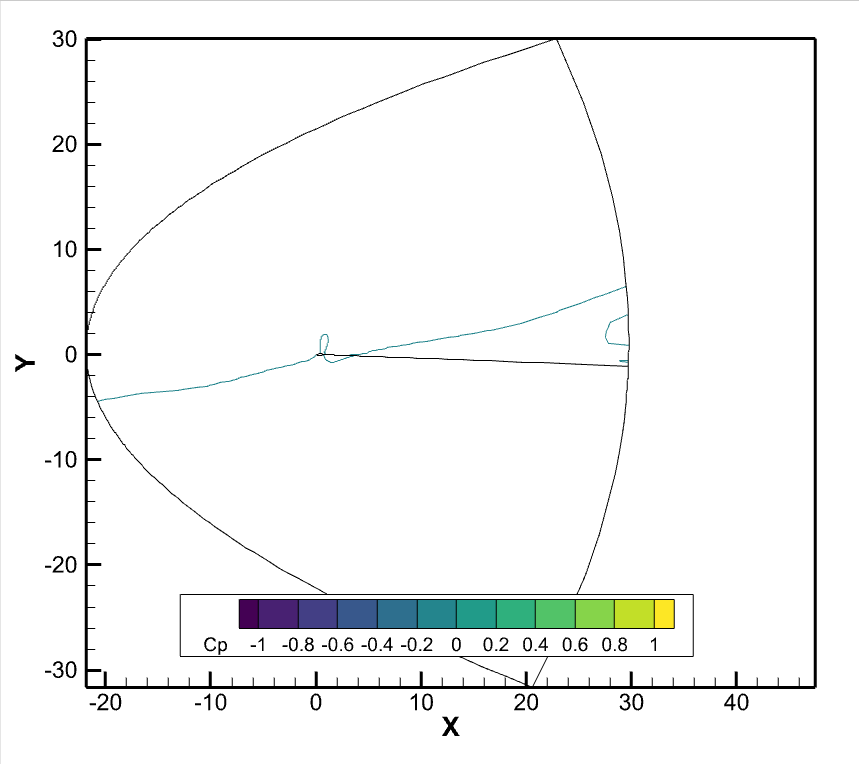
\includegraphics[width=\textwidth]{image/基压力分布图/双变量流场压力基2.png}
        \caption{第二POD模态}
    \end{subfigure}
    \begin{subfigure}[b]{0.32\textwidth}
        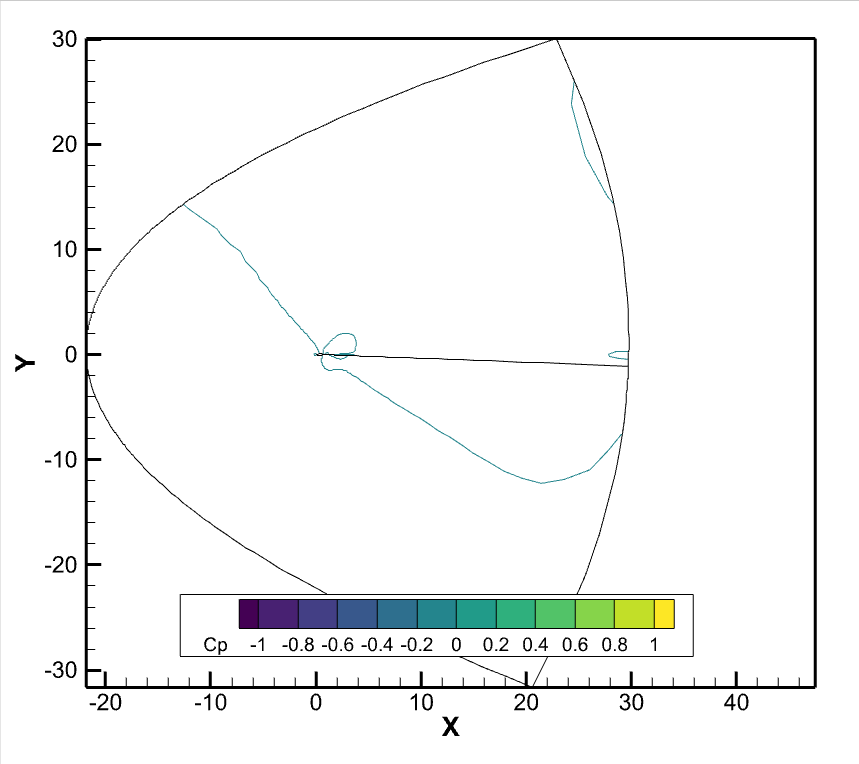
\includegraphics[width=\textwidth]{image/基压力分布图/双变量流场压力基3.png}
        \caption{第三POD模态}
    \end{subfigure}
    \caption{\songti 流场压力POD基模态}
    \label{fig:double_flow_pod_modes}
\end{figure}

\subsubsection{能量占比分析}

图 \ref{fig:double_flow_energy} 显示了流场压力POD基的能量占比。前九阶模态的累计能量占比达到95\%,表明POD方法能够有效提取流场压力分布的主要特征,用较少的模态即可实现高精度的流场重构。

\begin{figure}[H]
    \centering
    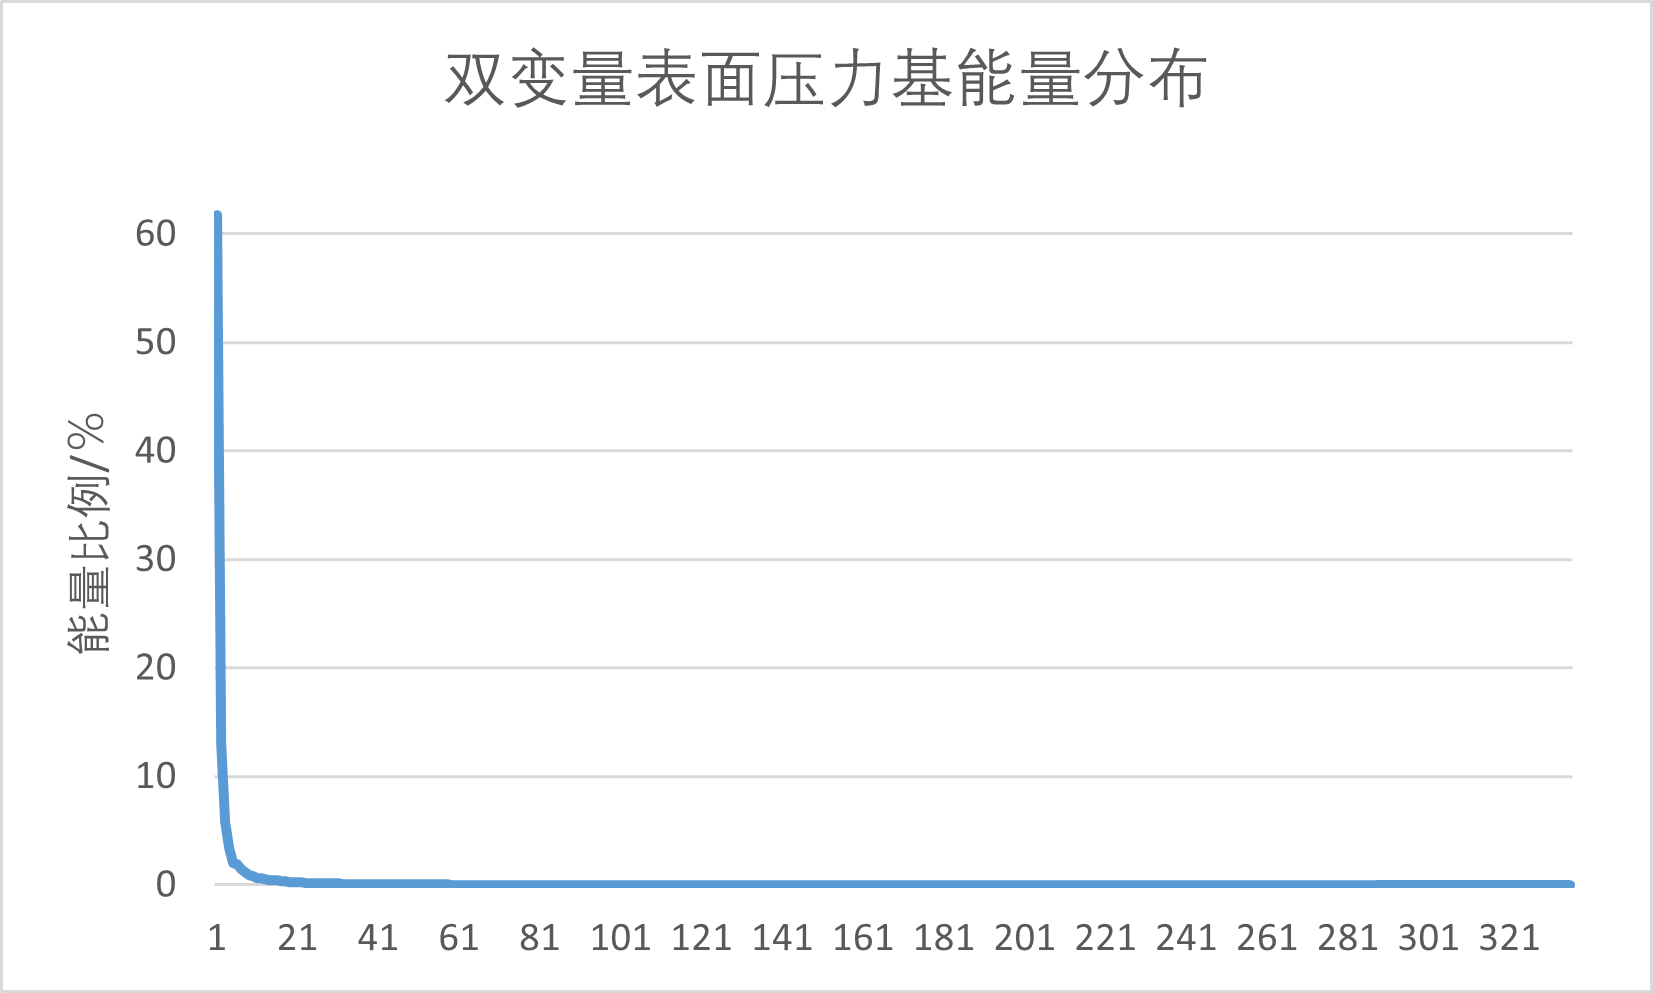
\includegraphics[width=0.8\linewidth]{image/基能量分布/双变量流场压力基能量分布.png}
    \caption{\songti 流场压力能量占比(前九阶模态占比95\%)}
    \label{fig:double_flow_energy}
\end{figure}

\subsubsection{插值验证对比}

图 \ref{fig:double_flow_validation} 对比了插值POD方法预测的流场压力分布与CFD模拟结果。在$\alpha=0.45^\circ$且$Mach=0.77^\circ$下,预测结果与CFD结果高度吻合。表 \ref{tab:double_flow_error} 显示,RMSE和MAE值均较低,皮尔逊相关系数接近1,表明插值POD方法具有较高的精度和可靠性。

\begin{figure}[H]
    \centering
    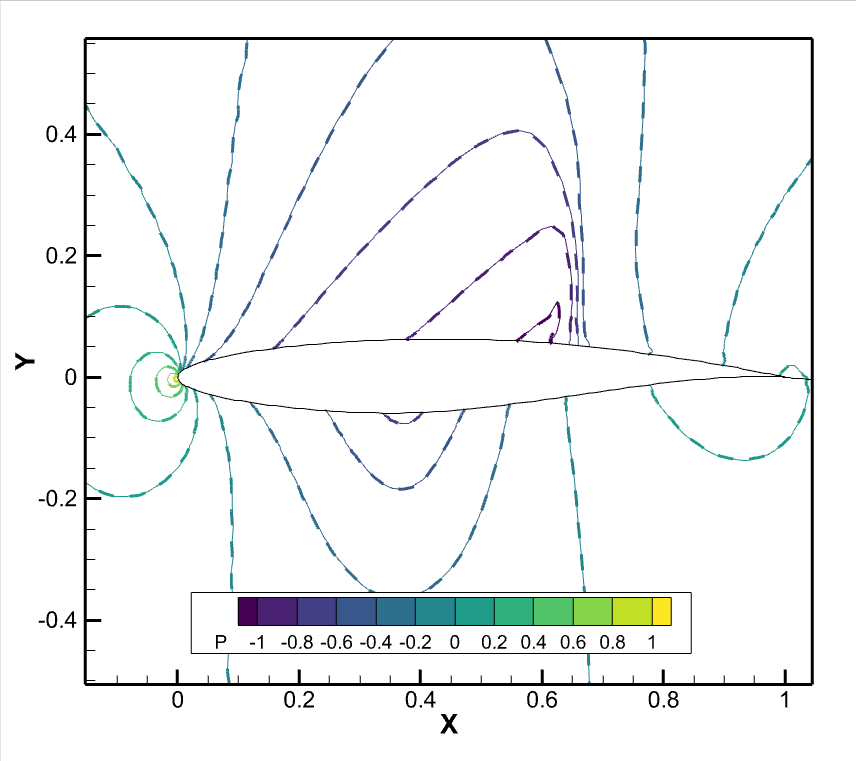
\includegraphics[width=0.8\textwidth]{0.45_0.77对比图.png}
    \caption{流场压力分布对比(实线:真实CFD结果;虚线:POD插值预测)}
    \label{fig:double_flow_validation}
\end{figure}

\begin{table}[H]
    \centering
    \caption{流场压力插值误差指标}
    \label{tab:double_flow_error}
    \begin{tabular}{lccc}
        \toprule
        工况 & RMSE($\times10^{-2}$) & MAE($\times10^{-2}$) & 相关系数 \\
        \midrule
        Mach=0.77,α=0.45° & 2.30 & 1.80 & 0.980 \\
        \bottomrule
    \end{tabular}
\end{table}


综上所述,双变量POD插值方法能够有效处理多参数变化情况下的流场重构问题,为复杂多变工况的流场分析提供了准确高效的解决方案。该方法通过构建低维POD基空间,结合三次样条插值技术,实现了对高维流场数据的高效压缩与精准重构,显著降低了计算成本,同时保持了较高的预测精度。

% ====================== 多变量POD-Kriging ======================
\section{多变量POD-Kriging插值算例}
\label{sec:multi_variable_pod_kriging}

本研究进一步探索了POD方法与Kriging插值相结合的多变量流场重构能力。针对NACA0012翼型,输入300组不同的19个设计变量及其对应的压力值数据,通过POD-Kriging方法实现对未知工况的高精度预测。

数据生成与预处理:
研究中使用了300组不同的设计变量组合,每组包含19个变量,用来表示翼型的几何参数变化。通过高保真CFD模拟获取对应的压力分布数据,确保了训练数据的质量和多样性。数据预处理流程包括:
\begin{itemize}
    \item {数据标准化}:对设计变量进行归一化处理,消除量纲差异
    \item {POD基函数生成}:利用SVD分解构建POD基函数空间,选择前19阶模态,保留超过99\%的能量特征
\end{itemize}

POD-Kriging模型训练:
基于预处理后的数据,构建POD-Kriging模型。
\begin{itemize}
    \item {POD降维}:将高维流场数据投影到低维POD基空间,提取主导模态系数
    \item {Kriging插值}:对POD系数进行Kriging插值建模,建立设计变量与POD系数之间的非线性映射关系:
    \begin{equation}
        \alpha_k(\boldsymbol{d}) = \sum_{i=1}^n w_i \mathcal{K}(\|\boldsymbol{d} - \boldsymbol{d}_i\|)
        \label{eq:kriging_model}
    \end{equation}
\end{itemize}

\subsection{表面压力分布分析}

\subsubsection{POD基模态分布}

图 \ref{fig:kriging_surface_pod_modes} 展示了表面压力分布的前三阶POD基模态。第一POD模态捕捉了表面压力分布的主要趋势,第二POD模态反映了压力分布的细微变化,第三POD模态则进一步捕捉了更高阶的细节特征。这些基模态共同构成了表面压力分布的低维特征空间。

\begin{figure}[H]
    \centering
    \begin{subfigure}[b]{0.32\textwidth}
        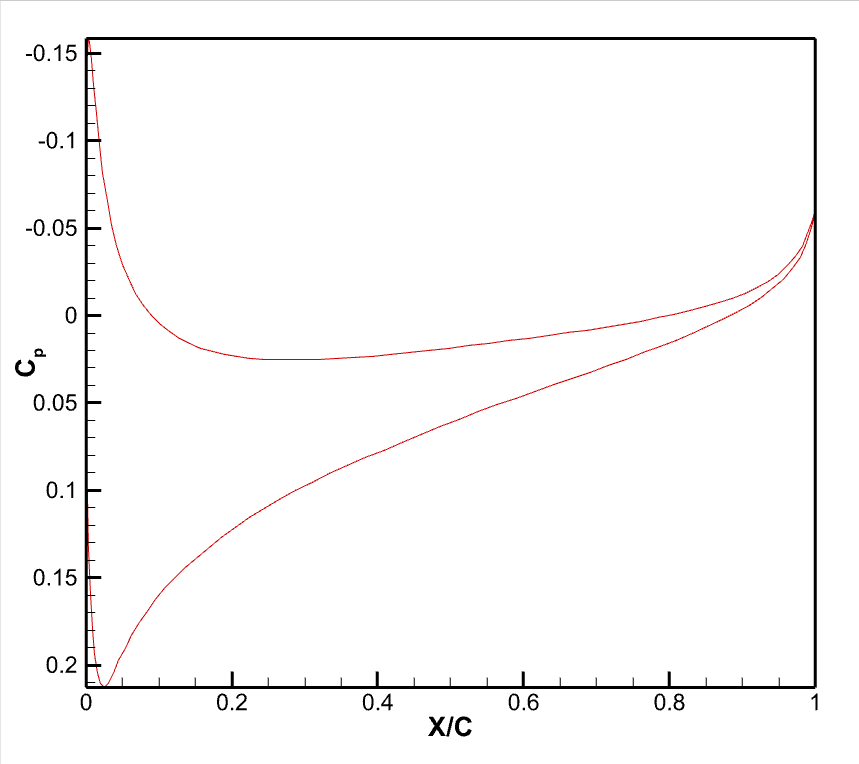
\includegraphics[width=\textwidth]{image/基压力分布图/多变量表面压力基1.png}
        \caption{第一POD模态}
    \end{subfigure}
    \begin{subfigure}[b]{0.32\textwidth}
        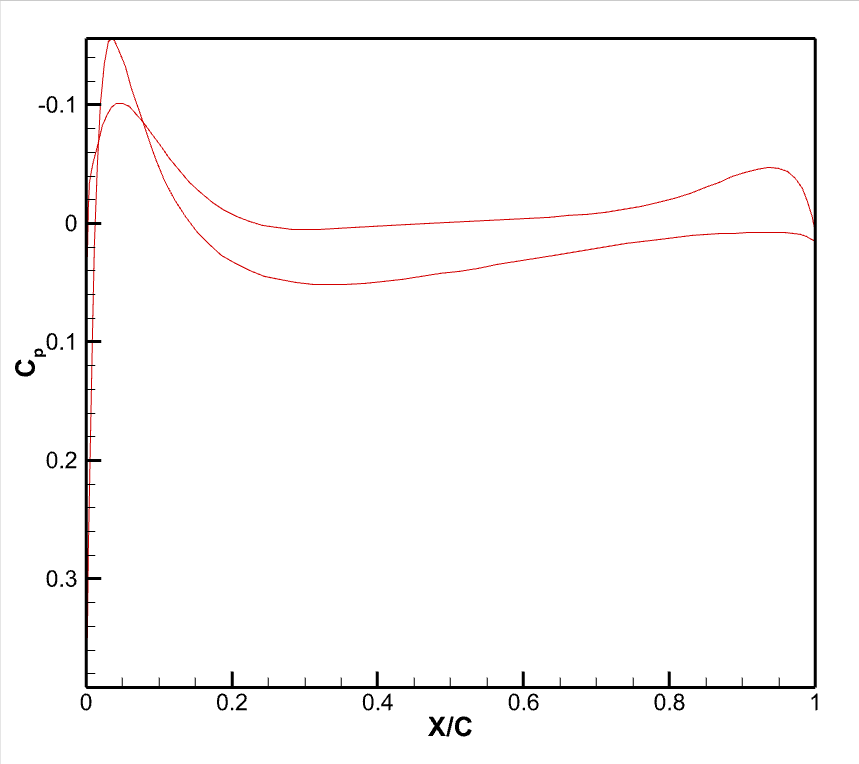
\includegraphics[width=\textwidth]{image/基压力分布图/多变量表面压力基2.png}
        \caption{第二POD模态}
    \end{subfigure}
    \begin{subfigure}[b]{0.32\textwidth}
        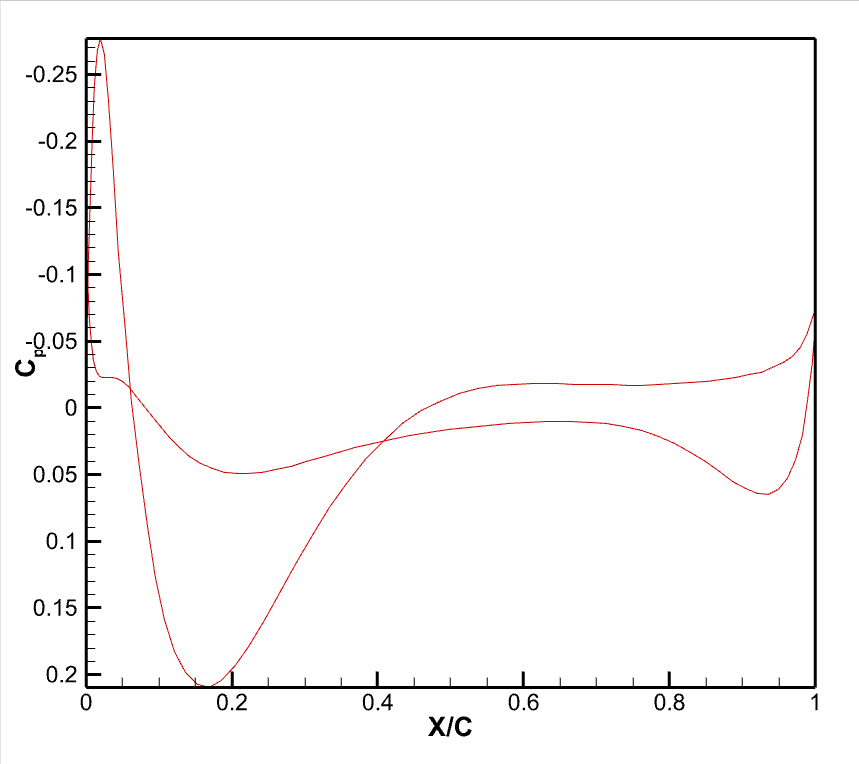
\includegraphics[width=\textwidth]{image/基压力分布图/多变量表面压力基3.png}
        \caption{第三POD模态}
    \end{subfigure}
    \caption{\songti 表面压力分布POD基模态}
    \label{fig:kriging_surface_pod_modes}
\end{figure}

\subsubsection{能量占比分析}

图 \ref{fig:kriging_surface_energy} 显示了表面压力POD基的能量占比。前两阶模态的累计能量占比达到95\%,表明POD方法能够有效提取表面压力分布的主要特征,用较少的模态即可实现高精度的流场重构。

\begin{figure}[H]
    \centering
    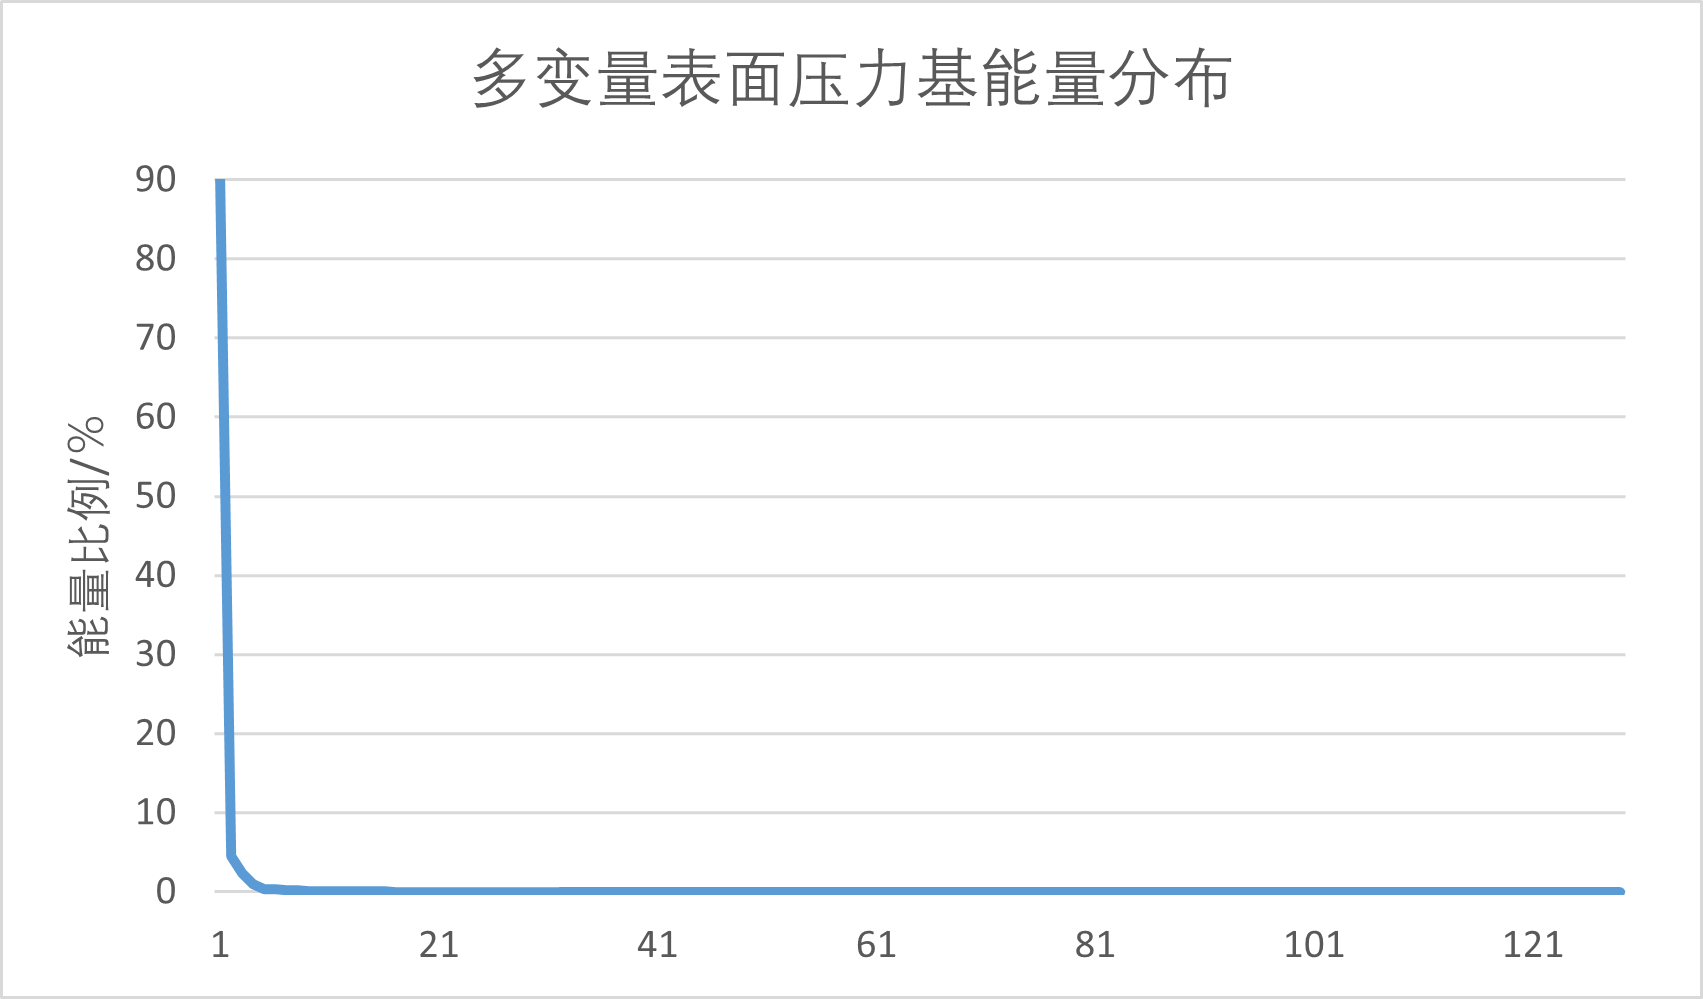
\includegraphics[width=0.8\linewidth]{image/基能量分布/多变量表面压力基能量分布.png}
    \caption{\songti 表面压力POD基能量占比(前两阶模态占比95\%)}
    \label{fig:kriging_surface_energy}
\end{figure}

\subsubsection{插值验证对比}

图 \ref{fig:kriging_surface_validation} 对比了POD-Kriging方法预测的表面压力分布与CFD模拟结果。随机生成一组19个设计变量的值,得到的预测结果与CFD结果高度吻合。表 \ref{tab:kriging_surface_error} 显示,RMSE和MAE值均较低,R$^2$值接近1,表明POD-Kriging方法具有较高的精度和可靠性。

\begin{figure}[H]
    \centering
    \begin{subfigure}[b]{0.45\textwidth}
        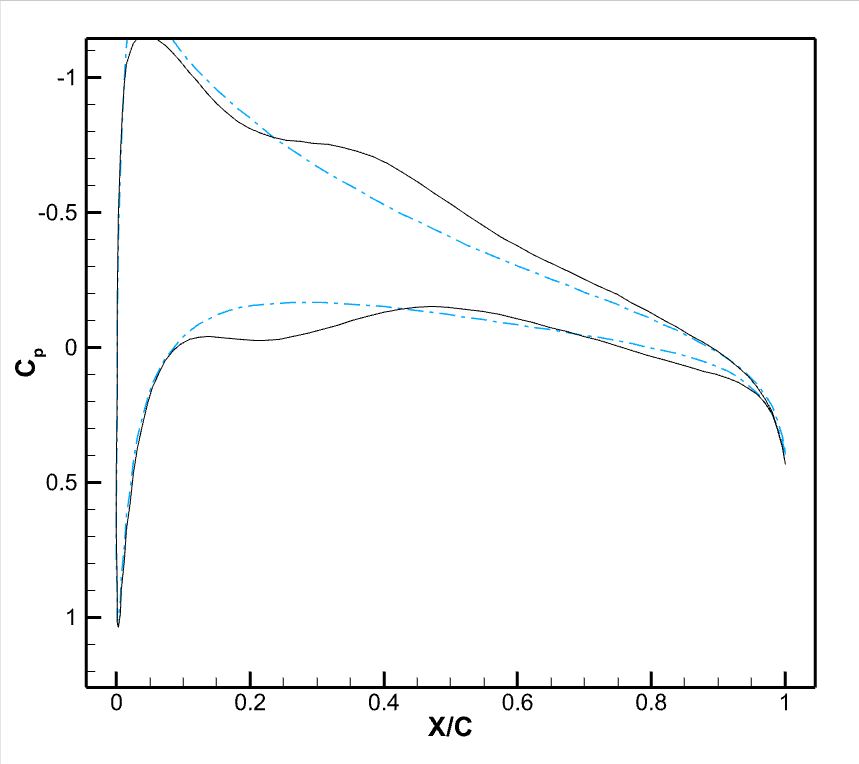
\includegraphics[width=\textwidth]{image/表面压力对比图/多变量第二组!.png}
        \caption{$\alpha=0.45^\circ$}
    \end{subfigure}
    \caption{\songti 表面压力插值验证(实线:CFD,虚线:预测)}
    \label{fig:kriging_surface_validation}
\end{figure}

\begin{table}[H]
    \centering
    \caption{多变量表面压力预测误差指标}
    \label{tab:kriging_surface_error}
    \begin{tabular}{lccc}
        \toprule
        \textbf{指标} & \textbf{RMSE} ($\times10^{-2}$) & \textbf{MAE} ($\times10^{-2}$) & \textbf{R$^2$} \\
        \midrule
        表面压力预测 & 3.12 & 2.48 & 0.956 \\
        \bottomrule
    \end{tabular}
\end{table}

\subsection{流场压力分布分析}

\subsubsection{POD基模态分布}

图 \ref{fig:kriging_flow_pod_modes} 展示了流场压力分布的前三阶POD基模态。第一POD模态捕捉了流场压力分布的主要趋势,第二POD模态反映了压力分布的细微变化,第三POD模态则进一步捕捉了更高阶的细节特征。这些基模态共同构成了流场压力分布的低维特征空间。

\begin{figure}[H]
    \centering
    \begin{subfigure}[b]{0.32\textwidth}
        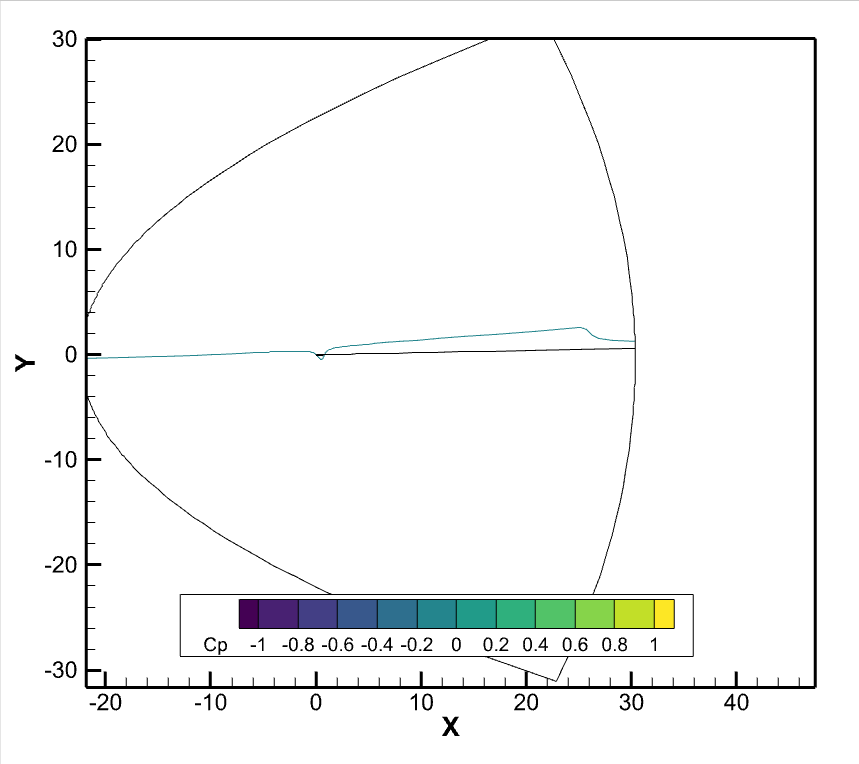
\includegraphics[width=\textwidth]{image/基压力分布图/多变量流场压力基1.png}
        \caption{第一POD模态}
    \end{subfigure}
    \begin{subfigure}[b]{0.32\textwidth}
        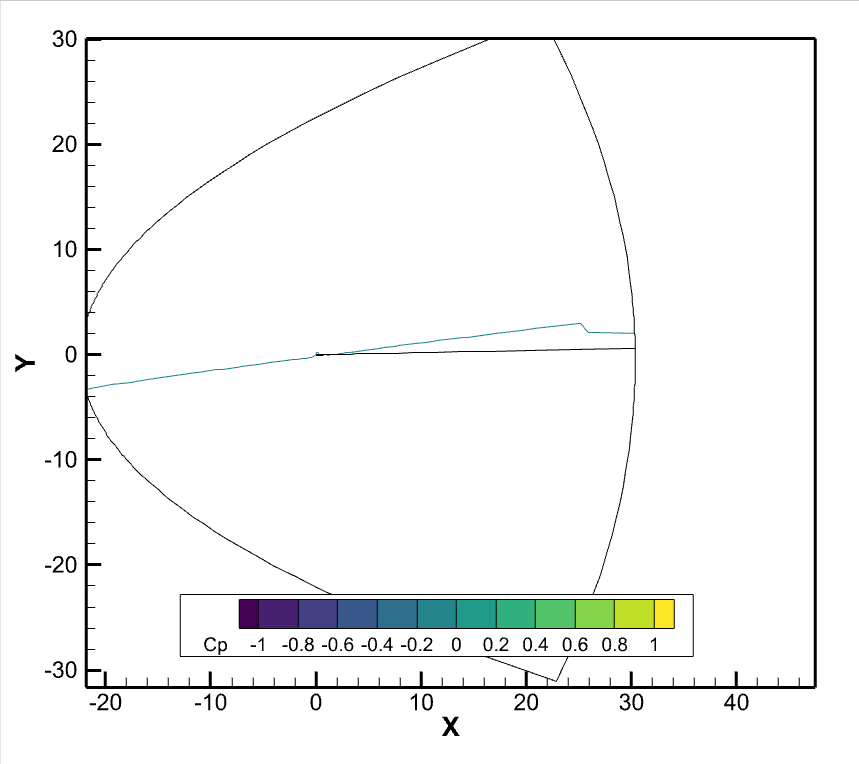
\includegraphics[width=\textwidth]{image/基压力分布图/多变量流场压力基2.png}
        \caption{第二POD模态}
    \end{subfigure}
    \begin{subfigure}[b]{0.32\textwidth}
        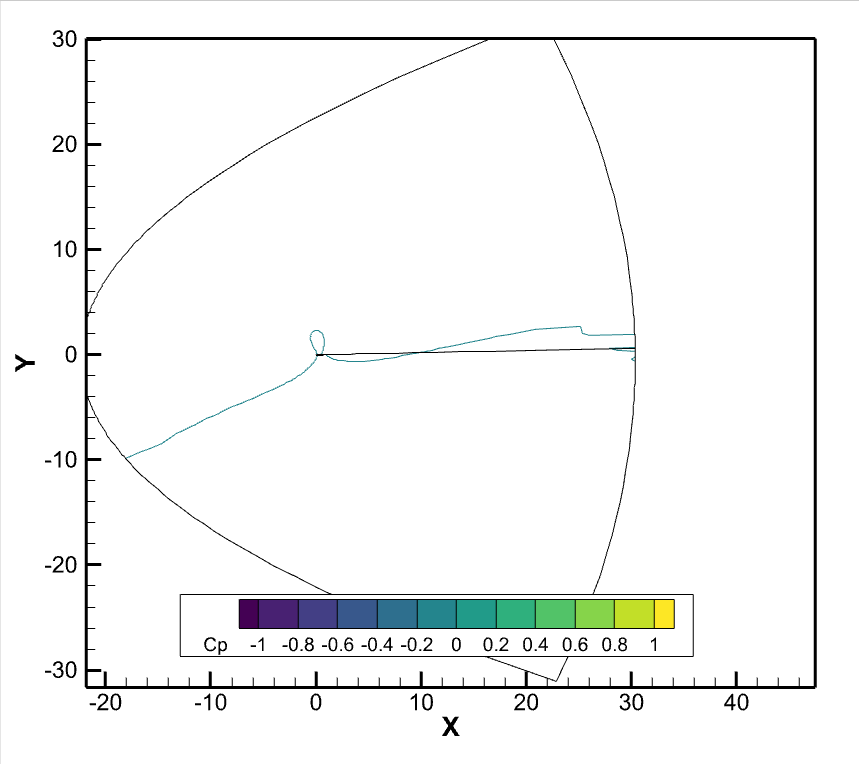
\includegraphics[width=\textwidth]{image/基压力分布图/多变量流场压力基3.png}
        \caption{第三POD模态}
    \end{subfigure}
    \caption{\songti 流场压力POD基模态}
    \label{fig:kriging_flow_pod_modes}
\end{figure}

\subsubsection{能量占比分析}

图 \ref{fig:kriging_flow_energy} 显示了流场压力POD基的能量占比。前九阶模态的累计能量占比达到95\%,表明POD方法能够有效提取流场压力分布的主要特征,用较少的模态即可实现高精度的流场重构。

\begin{figure}[H]
    \centering
    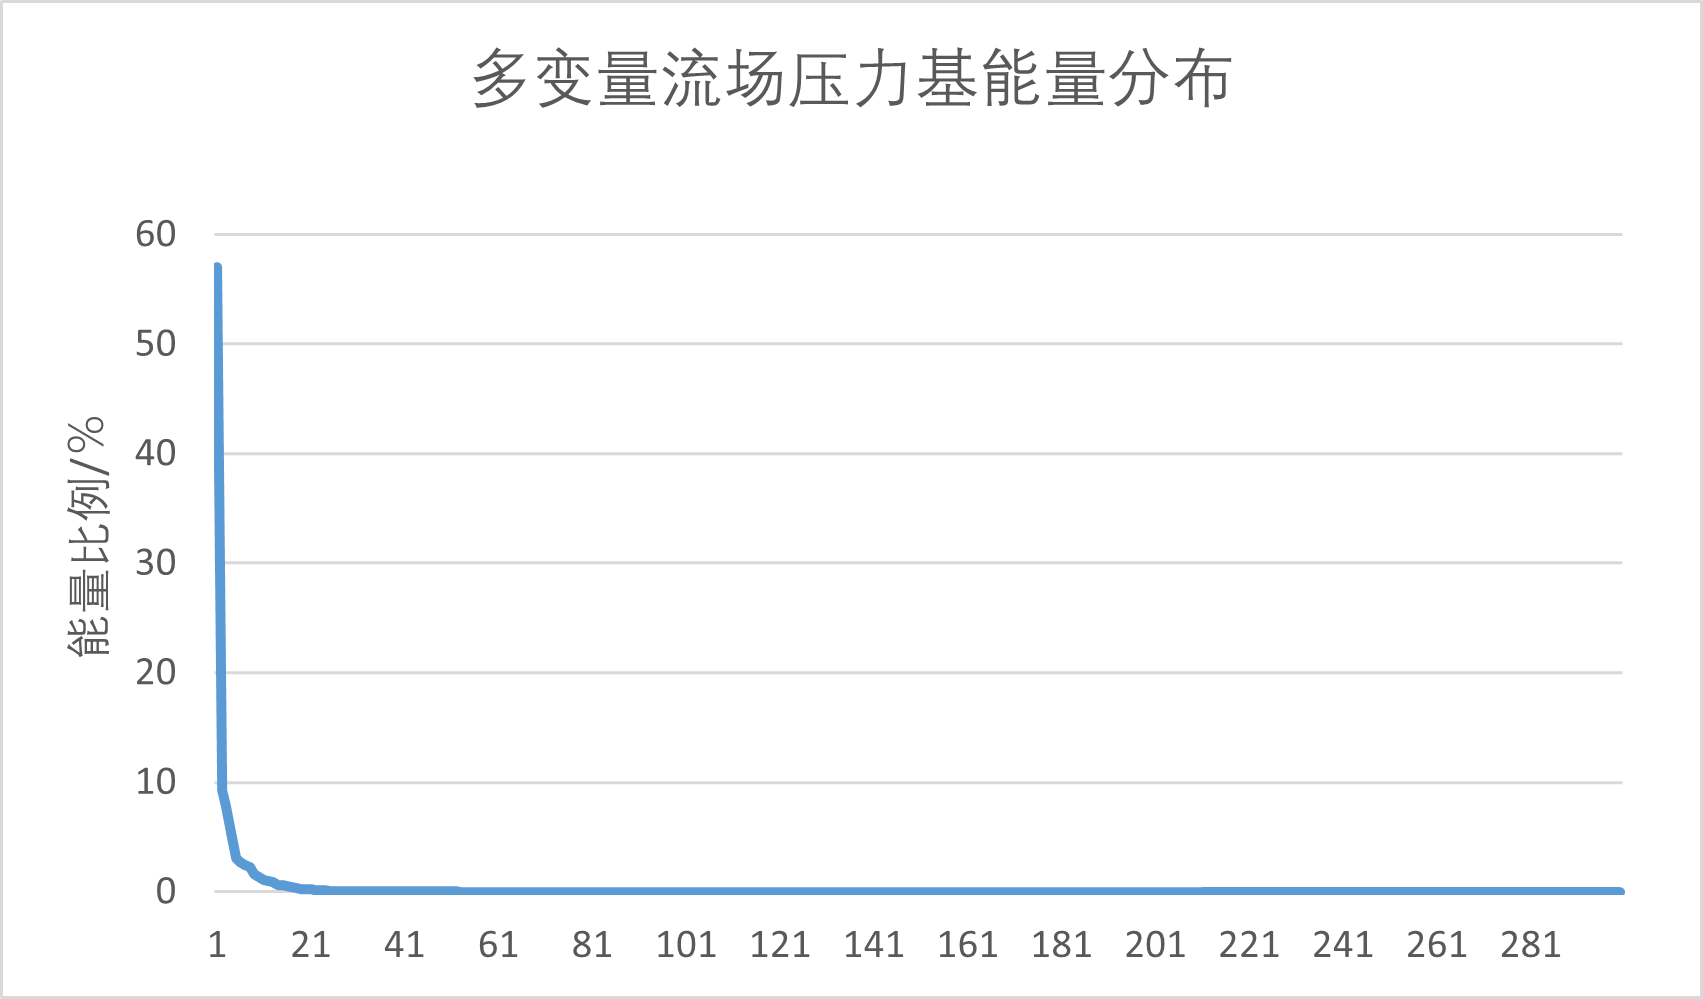
\includegraphics[width=0.8\linewidth]{image/基能量分布/多变量流场压力基能量分布.png}
    \caption{\songti 流场压力能量占比(前九阶模态占比95\%)}
    \label{fig:kriging_flow_energy}
\end{figure}

\subsubsection{插值验证对比}

图 \ref{fig:kriging_flow_validation} 对比了POD-Kriging方法预测的流场压力分布与CFD模拟结果。预测结果与CFD结果高度吻合。表 \ref{tab:kriging_flow_error} 显示,RMSE和MAE值均较低,R$^2$值接近1,表明POD-Kriging方法具有较高的精度和可靠性。

\begin{figure}[H]
    \centering
    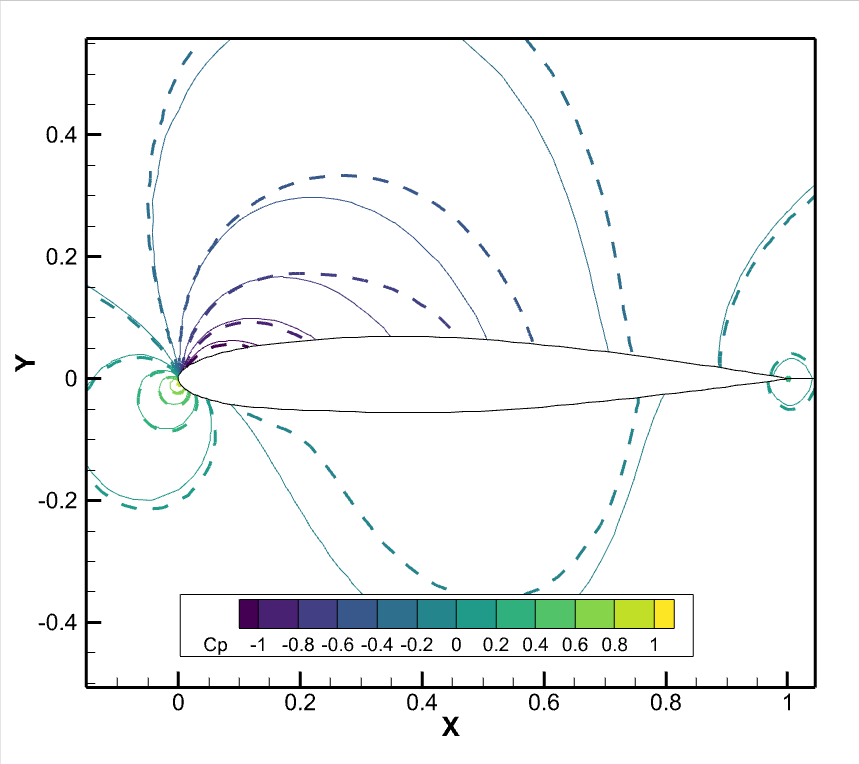
\includegraphics[width=0.8\textwidth]{image/多变量流场预测值与真实值对比结果图/多变量对比图2!.png}
    \caption{流场压力分布对比(实线:真实CFD结果;虚线:POD插值预测)}
    \label{fig:kriging_flow_validation}
\end{figure}

\begin{table}[H]
    \centering
    \caption{多变量流场压力预测误差指标}
    \label{tab:kriging_flow_error}
    \begin{tabular}{lccc}
        \toprule
        \textbf{指标} & \textbf{RMSE} ($\times10^{-2}$) & \textbf{MAE} ($\times10^{-2}$) & \textbf{R$^2$} \\
        \midrule
        压力场预测 & 3.25 & 2.56 & 0.952 \\
        \bottomrule
    \end{tabular}
\end{table}

该方法为多参数气动优化问题提供了新的解决方案,在保证精度的同时显著提升计算效率。未来可进一步研究自适应采样策略与深度Kriging模型的结合应用。